\documentclass[A4,10pt]{article}

%% DO NOT MODIFY THIS PREAMBLE
\usepackage{hyperref}
\usepackage{graphicx}
\usepackage{enumitem}
\setlist[itemize]{noitemsep}
\setlist[enumerate]{noitemsep}
\setlength{\parindent}{0cm}
\setlength{\parskip}{1ex}
\setlength{\columnsep}{25pt}

\textwidth=14cm
\textheight=23cm
\setlength{\unitlength}{0.5cm}
\setlength{\parindent}{0.0cm}
\setlength{\parskip}{0.5ex}
\raggedbottom
\sloppy
%\addtolength{\evensidemargin}{-5cm}
\addtolength{\oddsidemargin}{-3cm}
\addtolength{\topmargin}{-2cm}

\renewcommand{\baselinestretch}{1.2} 

%% ADD YOUR PACKAGES HERE
\usepackage{minted} % Add this line to include the minted package
\usepackage{siunitx} % Add this line to include the siunitx package
\usepackage{booktabs} % Add this line to include the booktabs package

\sloppy

% Your name
\author{Lukas Radovansky \\ Technische Universit\"at M\"unchen}

\title{Master Lab IoT}

% Date of your talk
\date{20.1.2025}


\begin{document}

\maketitle
\newpage
\tableofcontents
\newpage

\section{Background for grading (0.5 page)}
\begin{itemize}
	\item \textbf{General overview of your schedule including longer leave of absence (e.g., vacations) to explain missing data:}
	\begin{itemize}
		\item Couple of multiday trips during the semester.
		\item Christmas break from 15.12.2024 to 2.1.2025.
		\item Unnoticed MQTT broker issue from 13.1.2025 to 18.1.2025.
	\end{itemize}
	\item For more details, refer to Section~\ref{sec:data_reporting}.

	\item \textbf{Hardware problems:}
	\begin{itemize}
		\item At the beginning of the semester, I encountered a problem with my ESPs that couldn't maintain a stable connection to the FRITZBOX router.
		\item I spent a lot of time trying to fix the issue, but I couldn't find a solution.
		\item In the end, I asked my landlord to give me the router credentials to debug the issue, which he refused.
		\item Instead, he provided me with a small router that I connected to the FRITZBOX. This solved the issue, and I was able to continue with the project.
		\item However, the router was not able to maintain a stable connection all the time and sometimes had to be restarted.
	\end{itemize}

	\item \textbf{Credentials changed for the Digital Twin:}
	\begin{itemize}
		\item There were no credentials changed for the Digital Twin app.
	\end{itemize}
\end{itemize}

\section{Your setup at home (1 page)}

\begin{itemize}
	\item \textbf{Scale map and sensor placement:}
	\begin{itemize}
		\item Present the scale map with the placement of the sensor and the observed area.
	\end{itemize}
\end{itemize}

\begin{itemize}
	\item \textbf{Challenges from positioning:}
	\begin{itemize}
		\item The Sensor in the kitchen triggered false positives if the door to the kitchen were opened and someone was in the hallway. 
		\item The sensor placed in bathroom could be affected by the steam from the shower, however the device seems to survive the humidity well.
		\item I have deployed exactly one ESP with a Magnetic Switch and PIR sensor simultaneously in my apartment. It has been placed in the bedroom. The PIR sensor was pointing towards the bed area, and the magnetic switch was placed on the entrance door. The idea was to track the sleep time of the patient. If the doors remained open, the sensor was still active, and no bed area events were recorded. This was done on purpose because I know that every time the patient goes to sleep, he will close the door first.
	\end{itemize}
	\item \textbf{Setup information:}
	\begin{itemize}
		\item Sharing the flat with another person and a cat presented additional challenges in completing some tasks for this seminar.
		\item Occasionally, a third person (the landlord) would be present in the flat once or twice a week to work from the crossed-out room on the apartment map. The landlord also used the kitchen, where one of the PIR sensors was placed.
		\item Throughout the semester, we hosted guests on several occasions (4-5 times), which impacted the data collection process. The highest number of guests was five, during the weekend of December 12-15, 2024.
	\end{itemize}
\end{itemize}

\begin{figure}[H]
	\centering
	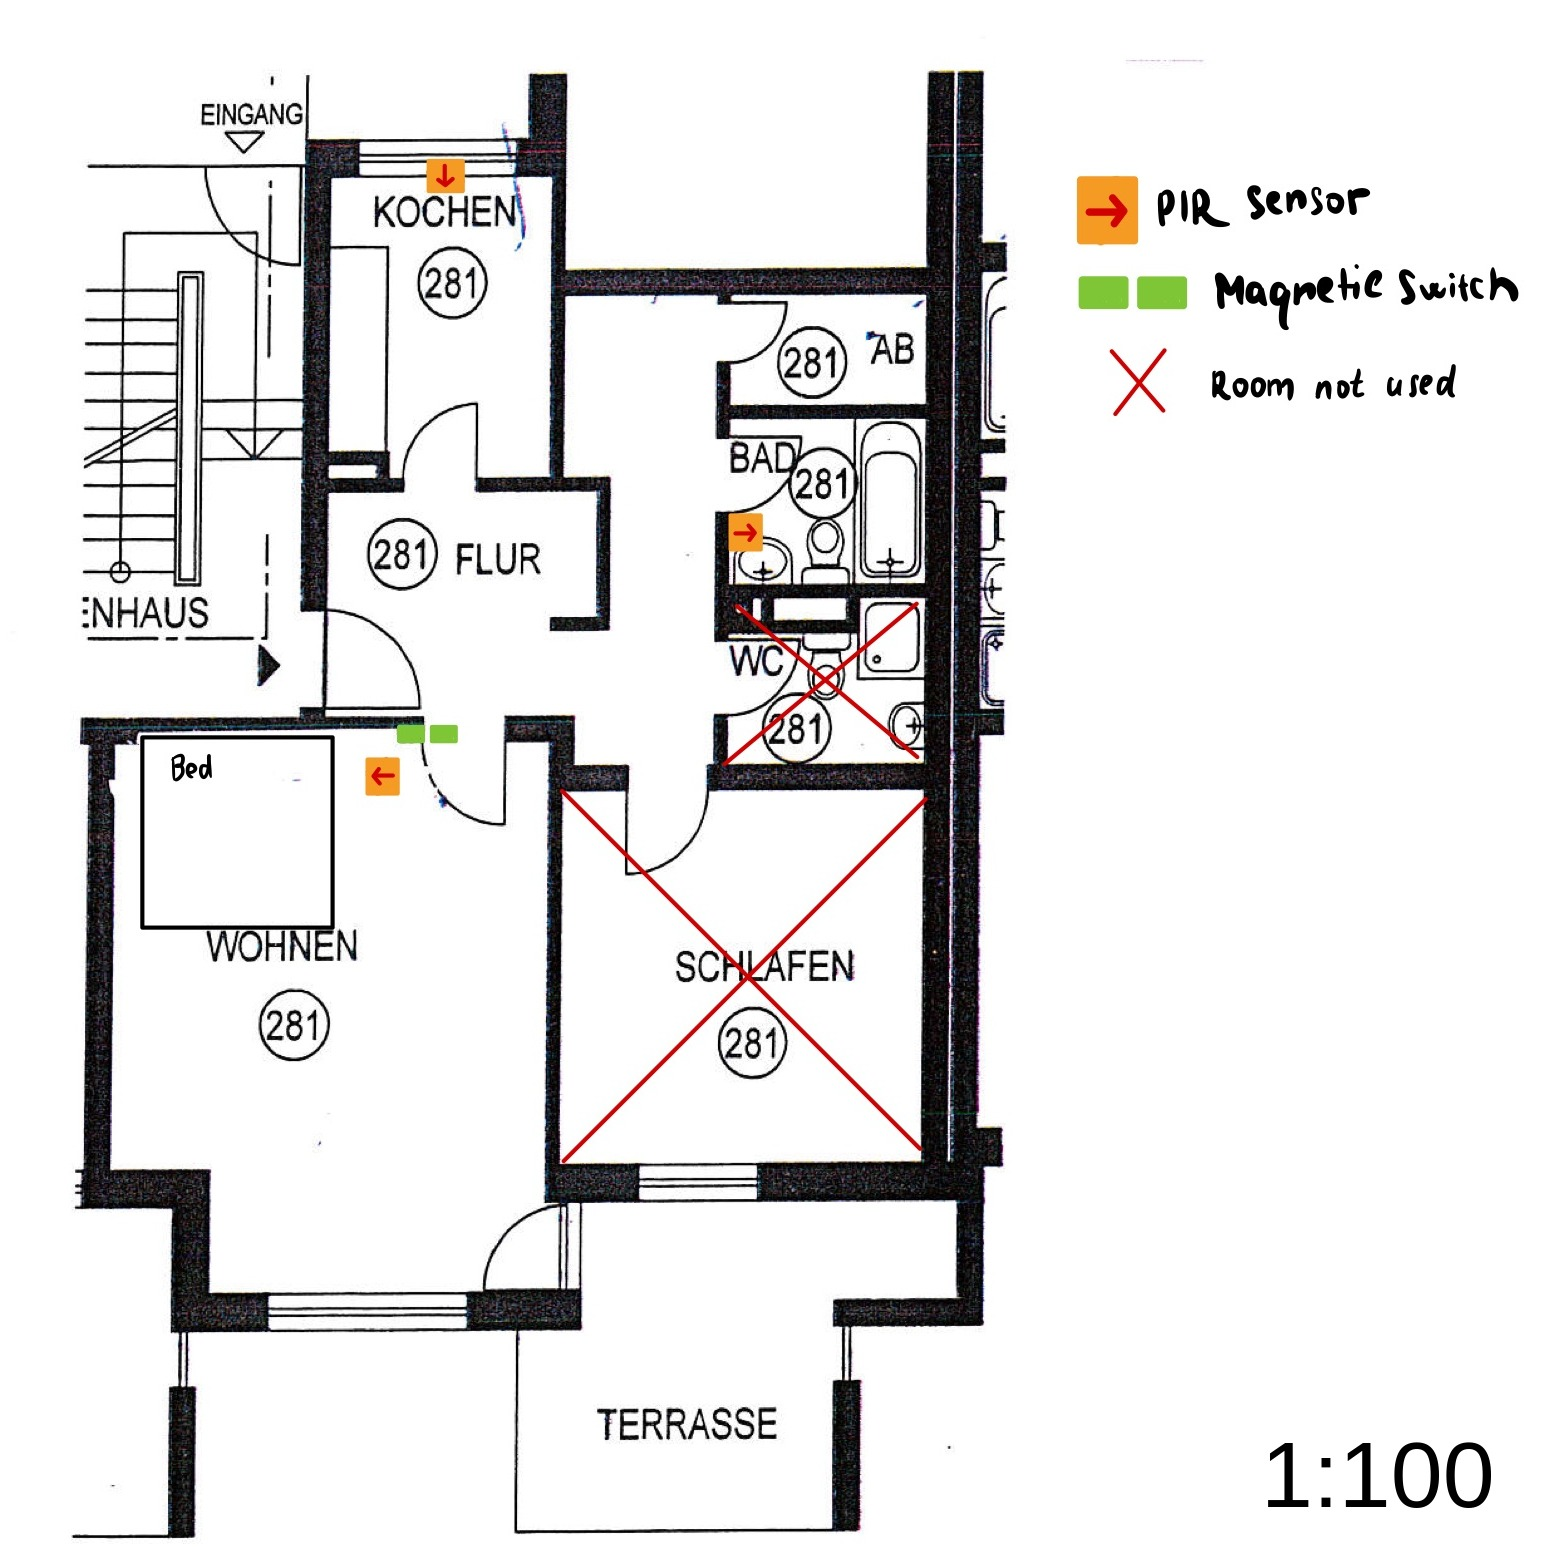
\includegraphics[width=1\textwidth]{grundriss.jpeg}
	\caption{Scale map illustrating the sensor placement and the monitored area. The scale is 1:100. Red arrows indicate the orientation of the PIR sensors. Crossed-out areas are not part of the rented section of the flat.}
	\label{fig:scale_map}
\end{figure}

\section{Sensor Development (10 pages)}

\subsection{Challenges (0.5p)}

\begin{itemize}
	\item \textbf{Describe any aspect to consider while grading that impacted the development of your code, such as: programming skills, difficulties in understanding concepts, etc.}
	\begin{itemize}
		\item I had limited experience with embedded systems programming, which required additional time to learn and understand the given tasks.
		\item I was also new to Docker and Kubernetes.
	\end{itemize}
\end{itemize}

\subsection{Sensor Integration (0.5p)}

\begin{itemize}
	\item \textbf{Integration of PIR and Magnetic Sensors}
	
	The integration of PIR sensors with a magnetic switch sensor was achieved through the following steps:

	\begin{enumerate}
		\item \textbf{Hardware Configuration:} 
		\begin{itemize}
			\item \textbf{PIR Sensor} connected to GPIO pin 27.
			\item \textbf{Magnetic Switch Sensor} connected to GPIO pin 33.
		\end{itemize}
		
		\item \textbf{GPIO Initialization:} 
		Both sensors are configured as RTC GPIOs with pull-down resistors to ensure stable low states when inactive.
		
		\begin{minted}[fontsize=\small]{c}
void configure_rtc_gpio() {
    // Initialize PIR sensor GPIO
    rtc_gpio_init(27);
    rtc_gpio_set_direction(27, RTC_GPIO_MODE_INPUT_ONLY);
    rtc_gpio_pulldown_en(27);
    
    // Initialize Magnetic Switch GPIO
    rtc_gpio_init(33);
    rtc_gpio_set_direction(33, RTC_GPIO_MODE_INPUT_ONLY);
    rtc_gpio_pulldown_en(33);
}
		\end{minted}
		
		\item \textbf{Wake-Up Configuration:} 
		Both sensors are set as wake-up sources using the EXT1 mechanism, allowing the ESP32 to wake from deep sleep when either sensor is triggered.
		\begin{minted}[fontsize=\small]{c}
uint64_t wakeup_pins = (1ULL << 27) | (1ULL << 33);
esp_sleep_enable_ext1_wakeup(wakeup_pins, ESP_EXT1_WAKEUP_ANY_HIGH);
		\end{minted}
		
		\item \textbf{Event Handling:} 
		Upon wake-up, the system identifies which sensor triggered the event and processes it accordingly.
		\begin{minted}[fontsize=\small]{c}
void handle_wakeup_reason(){
    if (wakeup_reason == ESP_SLEEP_WAKEUP_EXT1) {
        uint64_t status = esp_sleep_get_ext1_wakeup_status();
        if (status & (1ULL << 27)) {
            // Handle PIR sensor event
        }
        if (status & (1ULL << 33)) {
            // Handle Magnetic switch event
        }
    }
}
		\end{minted}
			\end{enumerate}
\end{itemize}

\subsection{Single Code for All Sensors (1p)}

\begin{itemize}
    \item \textbf{Generic Code Base for Multiple Sensors}
    
    \begin{itemize}
		\item \textbf{Describe how you achieved a generic code base for all your sensors devices. You can include code snippets.}
		\begin{itemize}
			\item Generic code for all devices was achieved by identifying the device based on its MAC address and configuring it accordingly.
			\item Each device needs to be specied in the `main.h` file with its device name, MAC address, ID, MQTT topic, security key, battery information availability, and room ID.
		\end{itemize}
	\end{itemize}

	\begin{minted}[fontsize=\small]{c}
//Struct definition for device information in main.h
/**
 * @brief Represents the configuration and metadata for a device.
 *
 * This struct is used to define the properties of an ESP device, including its
 * name, MAC address, ID, MQTT topic, security key, and whether battery information
 * is available. The struct can be used to identify devices and manage their specific
 * configurations within the system.
 */
 typedef struct {
    char* device_name;             // < Name of the device (e.g., "Living Room").
    uint8_t mac_address[6];        // < MAC address of the device (6 bytes).
    int device_id;                 // < Unique identifier for the device.
    char* device_topic;            // < MQTT topic for publishing device data.
    char* device_key;              // < Security key for authenticating with the MQTT broker.
    bool battery_info_available;   // < Indicates if the device provides battery information.
    char* room_id;                 // < Id of the room as named in the InFlux database.
} device_info_t;


// Example of definition of the device in main.h
// (name, mac adress, topic, key, battery info available, room_id)
#define ESP_DEVICE_1 {"Living Room", {0xEC, 0x62, 0x60, 0xBC, 0xE8, 0x50}, 4, 
"1/4/data", "key", true, "livingroombedarea"}

// Read the MAC address and identify the device in the main function:
uint8_t mac_address[6];
esp_read_mac(mac_address, ESP_MAC_WIFI_STA);
identify_device(mac_address);

// The implementation fo the identify_device function in main.c
identify_device(mac_address);
/**
 * @brief Identifies the current device based on its MAC address.
 *
 * Matches the MAC address of the device with the pre-configured device list in `main.h`.
 * Sets the device's ID, MQTT topic, security key, and battery information availability.
 *
 * @param mac_address Pointer to the MAC address array of the device.
 */
void identify_device(const uint8_t* mac_address) {
    for (int i = 0; i < sizeof(ESPs) / sizeof(ESPs[0]); ++i) {
        if (memcmp(mac_address, ESPs[i].mac_address, sizeof(ESPs[i].mac_address)) == 0) {
            // Copy the device info into this_device
            memcpy(&this_device, &ESPs[i], sizeof(device_info_t));
            // Logging
            ESP_LOGI("*", "*********** Device identified as %s", this_device.device_name);
            return;
        }
    }
    ESP_LOGI("*", "Device not recognized.");
}
    \end{minted}
    
\end{itemize}


\subsection{Wake-up stub (2p)}
\label{sec:wakeup_stub}

\subsubsection{Key Points}
\begin{itemize}
    \item \textbf{Sensor Trigger Filtering:} It checks if the sensors are newly triggered or still active. If the trigger is repetitive within a short time window, it returns to deep sleep without a full wake-up.
\begin{minted}[fontsize=\small]{c}
if (my_rtc_time_get_us() / 1000000 - last_wakeup_RTC <= SENSOR_INACTIVE_DELAY_IN_WAKE_UP_STUB_SEC) {
	last_wakeup_RTC = my_rtc_time_get_us() / 1000000;
	ets_delay_us(1000000); // Delay in microseconds.
	esp_wake_stub_set_wakeup_time(AUTOMATIC_WAKEUP_INTERVAL_SEC * 1000000);
	// Set stub entry, then go to deep sleep again.
	esp_wake_stub_sleep(&wake_stub);
}
last_wakeup_RTC = my_rtc_time_get_us() / 1000000;
\end{minted}
    \item \textbf{Conditional Full Wake-Up:} If the PIR event array is full, or if a magnetic switch triggers, the stub decides to fully boot into the main application.
    \item \textbf{Scheduled Timer Wake-Up:} Before returning to deep sleep, it sets a next wake-up timer, thus allowing periodic checks without fully waking the system each time. For this the variable \texttt{AUTOMATIC\_WAKEUP\_INTERVAL\_SEC} is used to set the next wake-up time.
\end{itemize}

\subsubsection{Timestamp Handling and Sending PIR Events in Time}
\begin{itemize}
    \item \textbf{RTC-Based Timing:} A helper function converts RTC counter ticks into microseconds, which the stub uses to get a ``local RTC time'' even in deep sleep.
	\begin{minted}[fontsize=\small]{c}
/**
 * @brief Retrieves the current RTC time in microseconds.
 *
 * This function reads the RTC time registers to obtain the current time.
 * It operates in the wake-up stub environment and uses low-level register access.
 *
 * @return Current RTC time in microseconds.
 */
RTC_IRAM_ATTR uint64_t my_rtc_time_get_us(void)
{
    SET_PERI_REG_MASK(RTC_CNTL_TIME_UPDATE_REG, RTC_CNTL_TIME_UPDATE);
    while (GET_PERI_REG_MASK(RTC_CNTL_TIME_UPDATE_REG, RTC_CNTL_TIME_VALID) == 0) {
        ets_delay_us(1); // Wait for RTC time to be valid.
    }
    SET_PERI_REG_MASK(RTC_CNTL_INT_CLR_REG, RTC_CNTL_TIME_VALID_INT_CLR);
    uint64_t t = READ_PERI_REG(RTC_CNTL_TIME0_REG);
    t |= ((uint64_t)READ_PERI_REG(RTC_CNTL_TIME1_REG)) << 32;

    uint32_t period = REG_READ(RTC_SLOW_CLK_CAL_REG);

    // Convert RTC clock cycles to microseconds.
    uint64_t now_us = ((t * period) >> RTC_CLK_CAL_FRACT);

    return now_us;
}
	\end{minted}
    \item \textbf{Unix Timestamp Calculation:} After each successful SNTP sync in the main app, we store:
        \begin{itemize}
            \item \texttt{rtc\_time\_at\_last\_sync}: RTC time in milliseconds at sync.
            \item \texttt{actual\_time\_at\_last\_sync}: Real Unix epoch time in milliseconds.
        \end{itemize}
\begin{minted}[fontsize=\small]{c}
// Extern declarations for time synchronization variables during wake up stub in main.h
// These variables will be stored in RTC memory to persist across deep sleep cycles
extern RTC_DATA_ATTR uint64_t rtc_time_at_last_sync;
extern RTC_DATA_ATTR uint64_t actual_time_at_last_sync;

// Storing reference times in the main app (after SNTP sync)
// main.c - after SNTP synchronization
actual_time_at_last_sync = get_current_time_in_ms();
rtc_time_at_last_sync = get_time_since_boot_in_ms();

uint64_t get_current_time_in_ms() {
    struct timeval now;
    gettimeofday(&now, NULL);
    return (uint64_t)(now.tv_sec) * 1000 + (now.tv_usec) / 1000; // Convert to milliseconds
}

uint64_t get_time_since_boot_in_ms() {
    return (my_rtc_time_get_us() / 1000); // Convert microseconds to milliseconds
}

\end{minted}
      The wake stub computes the \emph{actual} timestamp by adding the difference between current RTC time and \texttt{rtc\_time\_at\_last\_sync} to \texttt{actual\_time\_at\_last\_sync}.
\begin{minted}[fontsize=\small]{c}
// Computing actual timestamp in the wake stub:
void store_pir_event(void)
{
    // 1. Current RTC time in ms
    uint64_t rtc_time_now = my_rtc_time_get_us() / 1000;

    // 2. Calculate the time difference since last sync
    uint64_t rtc_time_diff = rtc_time_now - rtc_time_at_last_sync;

    // 3. Compute actual Unix timestamp in ms
    uint64_t actual_timestamp = actual_time_at_last_sync + rtc_time_diff;

    // Store the PIR event with the computed timestamp
    pir_events[pir_event_count].timestamp = actual_timestamp;
    // ...
}
\end{minted}
    \item \textbf{PIR Event Storage:}
	The PIR events are stored in an array of structs in RTC memory, until the array is full of a magnetic switch triggers a full wake-up or automatic wake-up interval is reached.
	\begin{minted}[fontsize=\small]{c}
/**
 * @brief Represents the struct for a PIR event
 *
 * This struct includes the timestamp of the event and the device information.
 */
 typedef struct {
    uint64_t timestamp;       // The actual Unix timestamp in milliseconds
    device_info_t device;     // Device information associated with the event
} PIR_Event_t;

// Define the maximum number of PIR events stored in RTC memory, the array 
// to store these events, and the counter for the events in main.h
extern RTC_DATA_ATTR uint32_t MAX_PIR_EVENTS;
extern RTC_DATA_ATTR PIR_Event_t pir_events[CONFIG_MAX_PIR_EVENTS];
extern RTC_DATA_ATTR int pir_event_count;
	\end{minted}
    \begin{itemize}
        \item If a PIR sensor wakes the device, the stub calls:
\begin{minted}[fontsize=\small]{c}
/**
 * @brief Stores a PIR event with the current timestamp and device information.
 *
 * Calculates the actual timestamp based on RTC time and synchronization data,
 * then stores the event in the PIR events array.
 */
 void store_pir_event(void)
{
	//...
    // Store the new event with the calculated actual timestamp.
    pir_events[pir_event_count].timestamp = actual_timestamp;
    // Since we cannot use memcpy in the wake-up stub, we manually copy each field.
    pir_events[pir_event_count].device.device_id = this_device.device_id;
    pir_events[pir_event_count].device.battery_info_available = this_device.battery_info_available;
    // Note: Assigning pointers directly as below is acceptable in the wake-up stub environment.
    pir_events[pir_event_count].device.device_name = this_device.device_name;
    pir_events[pir_event_count].device.device_topic = this_device.device_topic;
    pir_events[pir_event_count].device.device_key = this_device.device_key;
    pir_events[pir_event_count].device.room_id = this_device.room_id;
    // Copy MAC address manually.
    for (int i = 0; i < 6; i++) {
        pir_events[pir_event_count].device.mac_address[i] = this_device.mac_address[i];
    }
    // Increment the event count.
    pir_event_count++;
}
\end{minted}
        \item If \texttt{pir\_event\_count} hits its maximum, the stub forces a full wake to upload all stored events via MQTT.
    \end{itemize}
\end{itemize}

\subsection{Sending Battery RSOC (0.3p)}
\label{sec:battery_rsoc}

\begin{itemize}
    \item \textbf{RTC Timestamp Check:} The stub keeps a variable \texttt{last\_battery\_info\_time\_RTC}. On each wake, it checks if enough time has passed:
\begin{minted}[fontsize=\small]{c}
if ((my_rtc_time_get_us() / 1000000) - last_battery_info_time_RTC 
        >= BATTERY_INFO_INTERVAL_SEC) {
    last_battery_info_time_RTC = my_rtc_time_get_us() / 1000000;
    esp_default_wake_deep_sleep(); // Force main app to fully boot
}
\end{minted}
    \item Once awake, the main application reads the battery gauge and sends the RSOC (Remaining State of Charge) via MQTT. Since \texttt{last\_battery\_info\_time\_RTC} is in RTC memory, it persists through deep sleeps, ensuring strictly periodic RSOC uploads.
\end{itemize}


\subsection{Monday Problem (0.3p)}

\begin{itemize}[noitemsep]
    \item \textbf{What is the Monday problem?}\\
    The “Monday problem” refers to a situation where the Raspberry Pi (running the MQTT broker) is physically taken to class on Mondays, making the broker temporarily unreachable.

    \item \textbf{Approach to solving the Monday problem}\\
    To handle the broker’s unavailability, I introduced a boolean variable, \texttt{mqtt\_broker\_connected}, in \texttt{mqtt.c}. Whenever the device cannot connect to the broker, it skips sending data and retains the events in RTC memory. The next time the device fully wakes and finds the broker reachable, it sends all stored data.

    \item \textbf{Alternative attempts?}\\
    I did not attempt alternate solutions because the above approach—caching unsent events until reconnection—proved both straightforward and reliable.
\end{itemize}

\begin{minted}[fontsize=\small]{c}
// Wait for connection with a timeout of 10 seconds
EventBits_t bits = xEventGroupWaitBits(
    mqtt_event_group, CONNECTED_BIT, false, true, pdMS_TO_TICKS(10000)
);

if (bits & CONNECTED_BIT) {
    ESP_LOGI("mqtt", "Connected to MQTT\n");
} else {
    ESP_LOGI("mqtt", "Could not connect to MQTT broker\n");
    mqtt_broker_connected = false;
}

// Example of error handling for PIR events 
//(for battery information and magnetic switch data is the approach same)
if (!mqtt_broker_connected) {
    ESP_LOGI("PIR", "Cannot send stored PIR events, MQTT is not connected");
    return;
}
\end{minted}

 
\subsection{Power Consumption (1p)}
\label{sec:power_consumption}

\subsubsection{Power Consumption without Wake Up Stub}

\begin{itemize}
    \item \textbf{Phases of Code Execution (160\,MHz, No Light Sleep).} Each duty cycle includes five main phases:
    \begin{enumerate}
      \item \textbf{Boot:} \(\sim 30\,\si{\micro\watt\hour}\)
      \item \textbf{Wi-Fi Connection:} \(\sim 295\,\si{\micro\watt\hour}\)
      \item \textbf{Clock Synchronization (NTP):} \(\sim 125\,\si{\micro\watt\hour}\)
      \item \textbf{MQTT Connection \& Data Transmission:} \(\sim 31\,\si{\micro\watt\hour}\)
      \item \textbf{Deep Sleep:} \(\sim 0.1\,\si{\micro\watt\hour}\) (negligible)
    \end{enumerate}
    \noindent The total energy consumption per cycle (Boot + Wi-Fi + NTP + MQTT) is about \(481\,\si{\micro\watt\hour}\).
    
  \item \textbf{Typical Energy Use per Cycle.}
    \begin{itemize}
      \item \textbf{No Light Sleep (160\,MHz):} About 481\,\si{\micro\watt\hour} per cycle (Boot + Wi-Fi + NTP + MQTT).
      \item \textbf{Light Sleep (ALS 160\,MHz):} Around 435\,\si{\micro\watt\hour}.
      \item \textbf{Dynamic Frequency + ALS:} Can drop cycle energy to roughly 443\,\si{\micro\watt\hour} if clock sync is done less often.
    \end{itemize}

  \item \textbf{Measurement Variations.}
  Table~\ref{tab:power_summary} illustrates an example of minimum, maximum, mean, and standard deviation of per-cycle consumption (\si{\micro\watt\hour}) at different frequencies, with and without Automatic Light Sleep.

  \begin{table}[h!]
    \centering
    \caption{Power Consumption Summary (Per Cycle) for Various Frequencies}
    \label{tab:power_summary}
    \begin{tabular}{lcccc}
      \hline
      \textbf{Frequency (MHz)} & \textbf{Min (\si{\micro\watt\hour})} & \textbf{Max (\si{\micro\watt\hour})} & \textbf{Mean (\si{\micro\watt\hour})} & \textbf{Std (\si{\micro\watt\hour})} \\
      \hline
      80          & 420 & 510 & 465 & 27 \\
      160         & 460 & 520 & 481 & 20 \\
      240         & 490 & 585 & 540 & 27 \\
      160 + ALS   & 400 & 460 & 435 & 18 \\
      \hline
    \end{tabular}
  \end{table}

  \item \textbf{Battery Life Estimation.}  
  Let:
  \begin{itemize}
    \item $C_\mathrm{batt}$ = battery capacity in \si{\micro\watt\hour} (e.g.\ 1.4\,Ah at 3.7\,V $\approx$ 5{,}180{,}000\,\si{\micro\watt\hour}).
    \item $E_\mathrm{cycle}$ = measured energy consumption per cycle in \si{\micro\watt\hour}.
    \item $N_\mathrm{cycles}$ = number of cycles per day (e.g.\ 100).
  \end{itemize}
  Then the battery can sustain:
  \[
    \text{BatteryLife (cycles)} \;=\; \frac{C_{\mathrm{batt}}}{E_{\mathrm{cycle}}}.
  \]
  Over $N_\mathrm{cycles}$ per day, total days of operation is:
  \[
    \text{Days} \;=\; \frac{C_{\mathrm{batt}}}{E_{\mathrm{cycle}} \times N_{\mathrm{cycles}}}.
  \]
  For instance, with $C_{\mathrm{batt}}=5{,}180{,}000\,\si{\micro\watt\hour}$ and $E_{\mathrm{cycle}}=443\,\si{\micro\watt\hour}$ at 100 cycles/day, the device can run for roughly 117 days.
\end{itemize}

\subsubsection{Power Consumption with Wake Up Stub}

\begin{table}[h!]
    \centering
    \caption{Power Consumption per Wake Up Stub Cycle}
    \label{tab:power_summary}
    \begin{tabular}{lcccc}
      \hline
    \textbf{Min (\si{\micro\watt\hour})} & \textbf{Max (\si{\micro\watt\hour})} & \textbf{Mean (\si{\micro\watt\hour})} & \textbf{Std (\si{\micro\watt\hour})} \\
      \hline
      98 & 164 & 118 & 38 \\
    \end{tabular}
  \end{table}

\begin{itemize}
    \item The wake-up stub is used to significantly reduce the power consumption of the ESP32 per cycle. We will wake up and transmit the data only once every 10 cycles to transmit data. This approach avoids the need for a full wake-up cycle for every event.
    
    \item \textbf{Cycle Energy Consumption:}
    \begin{itemize}
      \item \textbf{No Wake-Up Stub:} 481\,\si{\micro\watt\hour}.
      \item \textbf{With Wake-Up Stub:} 
      \[
      \text{Average Energy per Cycle} = \frac{9 \times 118.8 + 1 \times 481}{10} = 156.02\,\si{\micro\watt\hour}.
      \]
    \end{itemize}
    
    \item \textbf{Energy Savings:}
    \[
    E_{\mathrm{saving}} = 481 - 156.02 = 324.98\,\si{\micro\watt\hour}.
    \]
    Over 100 cycles:
    \[
    E_{\mathrm{total\_saving}} = 324.98 \times 100 = 32{,}498\,\si{\micro\watt\hour}.
    \]
\end{itemize}

Battery Life Calculation with Wake-Up Stub

\textbf{Given:}
\begin{itemize}
    \item Battery capacity, \( C_\mathrm{batt} = 5{,}180{,}000 \, \si{\micro\watt\hour} \)
    \item Energy per cycle with wake-up stub, \( E_{\mathrm{cycle}} = 156.02 \, \si{\micro\watt\hour} \)
    \item Number of cycles per day, \( N_\mathrm{cycles} = 100 \)
\end{itemize}

\textbf{Formula for Battery Life (in days):}
\[
\text{Days} = \frac{C_{\mathrm{batt}}}{E_{\mathrm{cycle}} \times N_{\mathrm{cycles}}}
\]

\textbf{Substituting the values:}
\[
\text{Days} = \frac{5{,}180{,}000}{156.02 \times 100}
\]
\[
\text{Days} = \frac{5{,}180{,}000}{15{,}602} \approx 331.4 \, \text{days}
\]

\textbf{Conclusion:} With the wake-up stub, the battery will last approximately \textbf{331 days} at 100 cycles per day.

\subsection{Limitations (0.5p)}

The final solution meets the core requirements. However, it can be improved in the following ways:
\begin{itemize}
    \item Currently, only simple logic is used to filter repeated sensor triggers (If the patient stays active next to the sensor). More sophisticated signal filtering could prevent repeated events.
    \item The application relies heavily on RTC memory for event storage. If the memory becomes full, older events risk being overwritten. An SD card or external storage could help preserve data when connectivity is lost.
    \item Adding more sensors might require dynamic sensor configuration and more sophisticated scheduling for wake-ups. Current solution is tailored to a predefined sensors.
\end{itemize}

\subsection{Code Structure} The project uses a standard ESP-IDF layout under the \texttt{main} folder, as shown below:
\begin{verbatim}
|- CMakeLists.txt
|- main
|   |- CMakeLists.txt
|   |- component.mk
|   |- gauge.c / gauge.h       (Battery gauge handling)
|   |- main.c / main.h         (Main application logic)
|   |- mqtt.c / mqtt.h         (MQTT client setup and event publishing)
|   |- rtc_wake_stub.c / .h    (Wake-up stub logic for low-power triggers)
|   |- sntp.c / sntp.h         (SNTP initialization and time synchronization)
|   |- wifi.c / wifi.h         (Wi-Fi provisioning, connection, event handling)
\end{verbatim}

\noindent Below is a brief overview of the files:
\begin{itemize}
    \item \texttt{main.c, main.h}: Contains application entry-point (\texttt{app\_main}), handles device identification, event loops, power configuration, and sets up wake-up sources.
    \item \texttt{rtc\_wake\_stub.c, .h}: Implements the minimal RTC wake-up stub, including time checks, sensor event handling, and re-entry into deep sleep if needed.
    \item \texttt{wifi.c, wifi.h}: Initializes and manages the Wi-Fi connection (WPA2, SSID/password, IP assignment).
    \item \texttt{mqtt.c, mqtt.h}: Sets up MQTT connectivity, handles message publishing (e.g., PIR events, battery status).
    \item \texttt{sntp.c, sntp.h}: Configures SNTP for accurate time synchronization with NTP servers.
    \item \texttt{gauge.c, gauge.h}: Includes battery gauge drivers to measure voltage and state-of-charge (RSOC).
\end{itemize}

 
\subsection{Data Reporting (2p)}
\label{sec:data_reporting}

\begin{itemize}
    \item \textbf{Proof of Continuous Deployment:}
    Figure~\ref{fig:all_sensors_data} provides an overarching view of all recorded sensor data (kitchen, living room, bathroom). Despite certain offline periods (data gaps), the devices generally remained deployed and actively reported when connected and powered.

\begin{figure}[H]
    \centering
    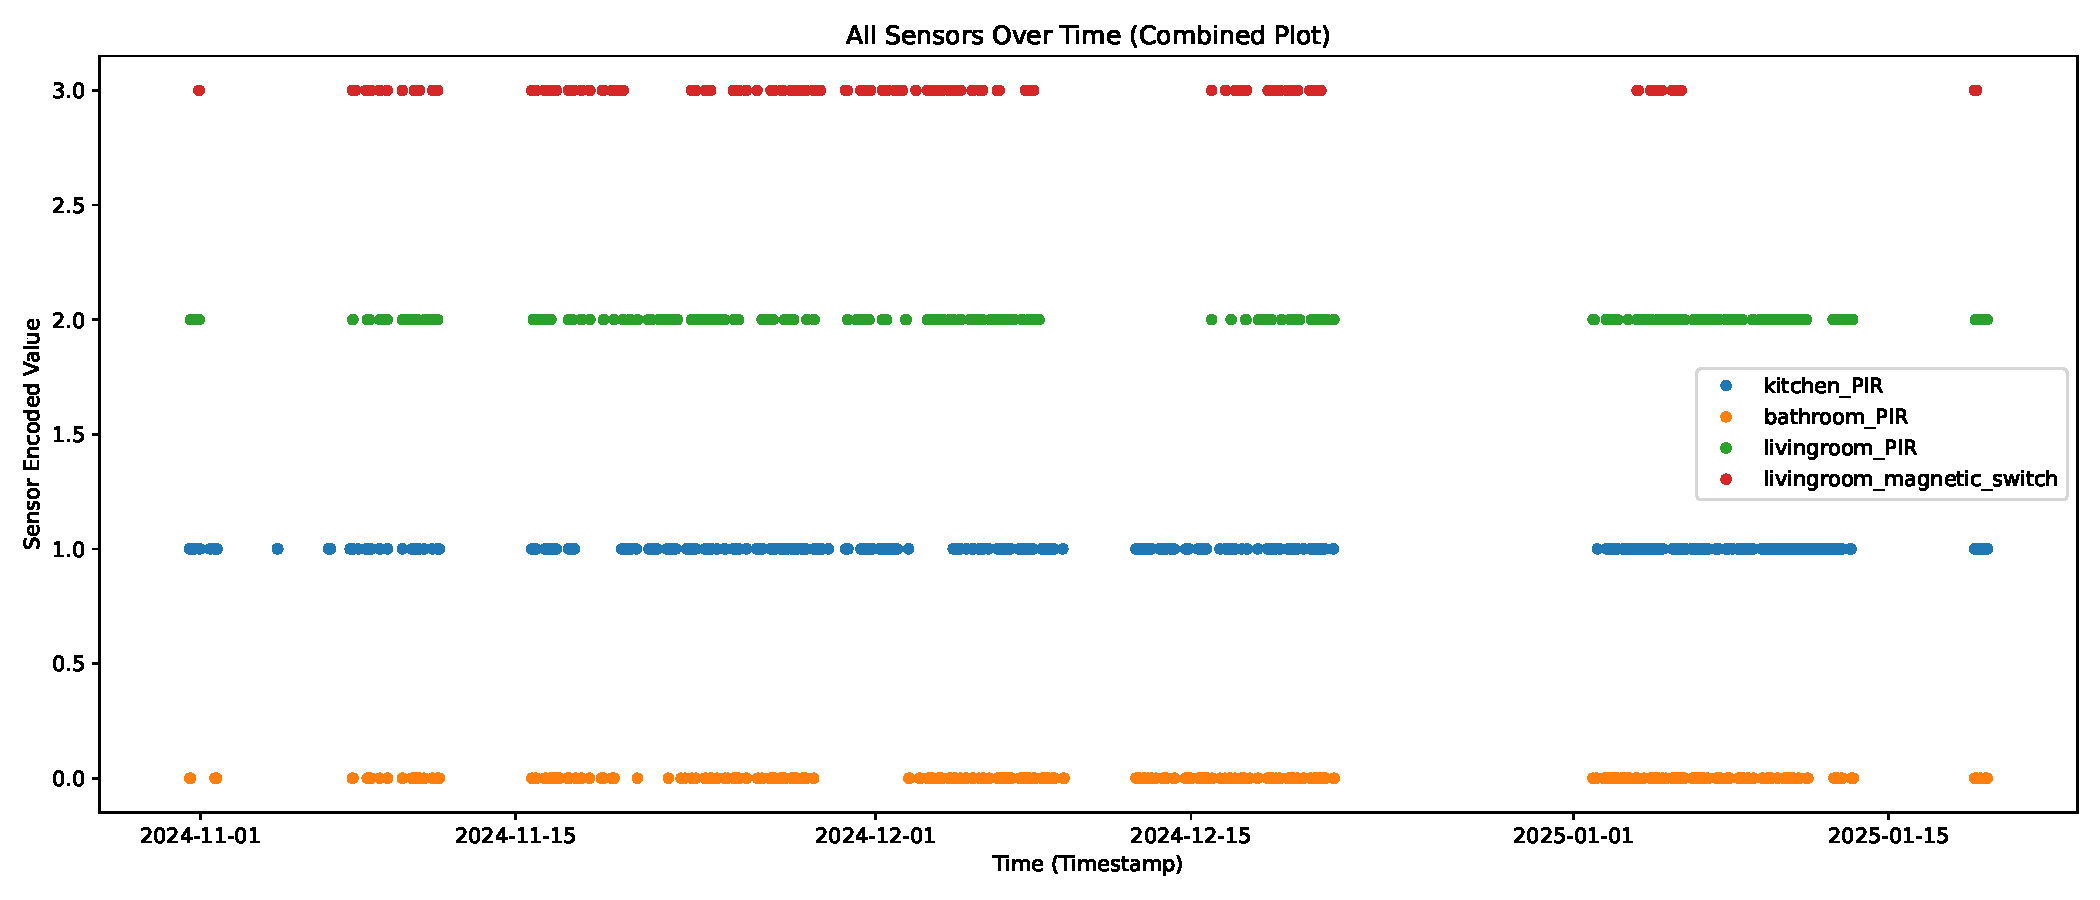
\includegraphics[width=1.15\textwidth]{all_sensors_data.pdf}
    \caption{Consolidated view of sensor data (kitchen, living room, bathroom). Each symbol corresponds to a different sensor.}
    \label{fig:all_sensors_data}
\end{figure}

    \item \textbf{Battery Usage Graphs:}
    Figures~\ref{fig:kitchen_battery} and~\ref{fig:livingroom_battery} show examples of kitchen and living room battery levels over time. The bathroom ESP32 did not support battery monitoring.

    \begin{figure}[H]
        \centering
        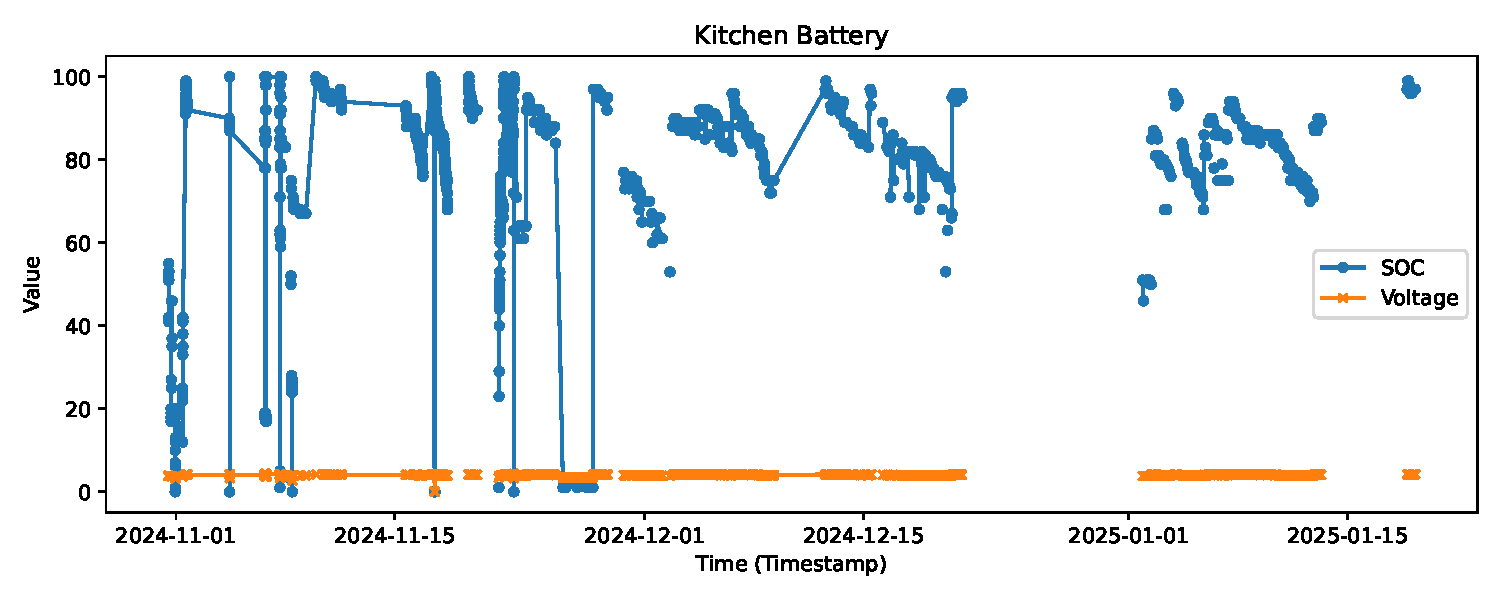
\includegraphics[width=1.15\textwidth]{kitchen_battery.pdf}
        \caption{Kitchen device battery usage and PIR event timestamps.}
        \label{fig:kitchen_battery}
    \end{figure}

    \begin{figure}[H]
        \centering
        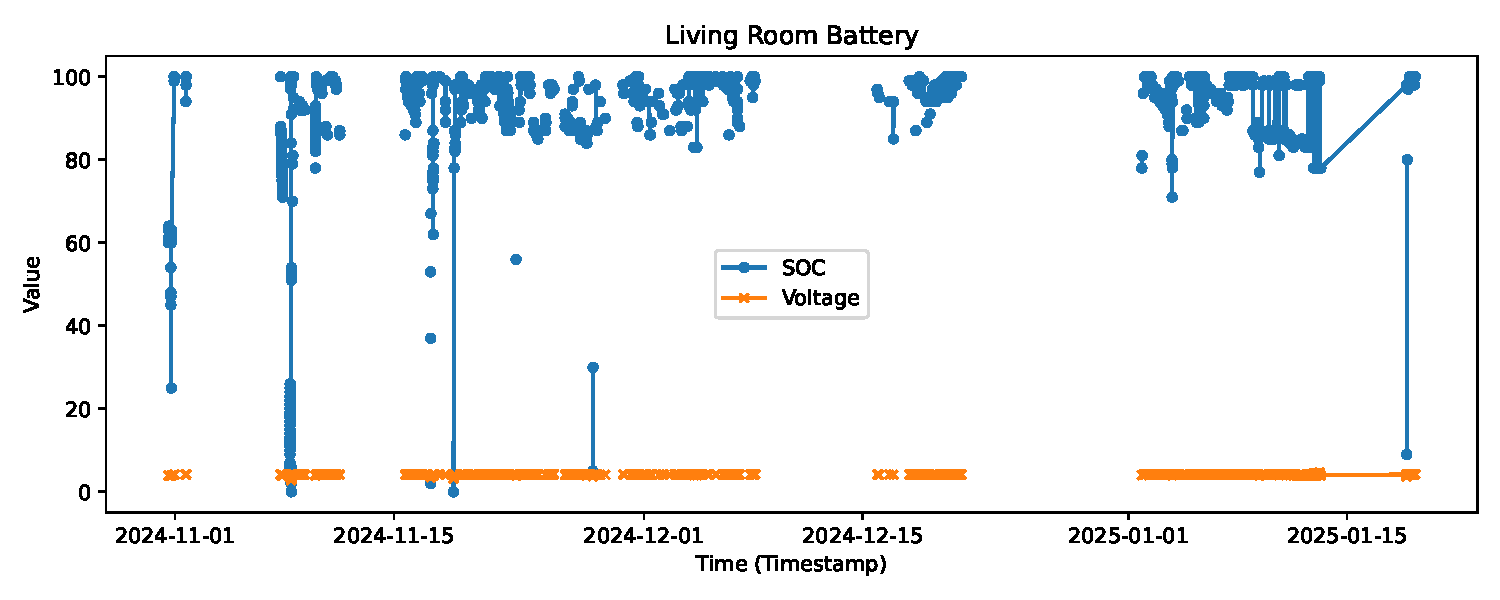
\includegraphics[width=1.15\textwidth]{livingroom_battery.pdf}
        \caption{Living Room device battery usage and PIR event timestamps.}
        \label{fig:livingroom_battery}
    \end{figure}

	\subsubsection{Data Gaps Overview}
	\label{sec:data_gaps}
	
	Despite good coverage, there were multi-day outages for each sensor due to initial deployment issues, holiday breaks multi-day trips and unnoticed issue with MQTT broker. Tables~\ref{tab:pir_gaps} and~\ref{tab:magnetic_gaps} summarize these periods, including reasons.
	
	\begin{table}[ht!]
	\centering
	\caption{Data Gaps for PIR Sensors}
	\label{tab:pir_gaps}
	\begin{tabular}{lllll}
	\hline
	\textbf{Sensor}            & \textbf{Gap Start}      & \textbf{Gap End}       & \textbf{Duration} & \textbf{Reason}              \\
	\hline
	\multicolumn{5}{l}{\textbf{PIR Sensors Gaps}} \\
							   & 2024-11-01 17:53        & 2024-11-04 09:55       & $\sim3$ days      & Initial deployment           \\
							   & 2024-11-04 10:35        & 2024-11-06 16:25       & $\sim2$ days      & Initial deployment           \\
							   & 2024-11-11 14:48        & 2024-11-15 17:14       & $\sim4$ days      & Initial deployment           \\
							   & 2024-11-17 14:50        & 2024-11-19 17:10       & $\sim2$ days      & Short trip                   \\
							   & 2024-12-09 07:30        & 2024-12-12 13:30       & $\sim3$ days      & Pre-Christmas break          \\
							   & 2024-12-16 08:08        & 2025-01-02 01:21       & $\sim16$ days     & Christmas break              \\
							   & 2025-01-13 07:54        & 2025-01-18 19:34       & $\sim5$ days      & Unnoticed MQTT broker issue               \\
	\end{tabular}
	\end{table}
	
	\begin{table}[ht!]
	\centering
	\caption{Data Gaps for \texttt{livingroom\_magnetic\_switch}}
	\label{tab:magnetic_gaps}
	\begin{tabular}{llll}
	\hline
	\textbf{Gap Start}      & \textbf{Gap End}        & \textbf{Duration} & \textbf{Reason}             \\
	\hline
	2024-10-31 22:42        & 2024-11-07 18:10        & $\sim7$ days      & Initial deployment          \\
	2024-11-11 12:57        & 2024-11-15 17:17        & $\sim4$ days      & Initial deployment          \\
	2024-11-17 18:48        & 2024-11-22 19:36        & $\sim3$ days      & Short trip                  \\
	2024-12-08 00:18        & 2024-12-15 22:10        & $\sim8$ days      & Unnoticed cable disconnection         \\
	2024-12-16 18:45        & 2025-01-03 19:49        & $\sim16$ days     & Christmas break             \\
	2025-01-05 18:48        & 2025-01-18 19:32        & $\sim13$ days     & Unnoticed MQTT broker issue + cable disconnection \\
	\hline
	\end{tabular}
	\end{table}
	
	\noindent
	\textbf{Comment on Gaps.} 
	These offline intervals primarily occurred around the initial deployment period (before mid-November), the Christmas holiday (late December), and unnoticed MQTT broker issue in January. Once reconnected, the sensors resumed normal operation, uploading new PIR or magnetic switch events to the MQTT broker.
	
\end{itemize}

\pagebreak
\section{Digital Twin (17 pages)}

\subsection{Event-driven Programming (1p)}

\begin{itemize}
    \item \textbf{Challenges with a Distributed, Event-driven System} \\
    I was already comfortable with Python and machine learning, but I had limited experience with distributed systems, containers (like Docker), and orchestration platforms (like Kubernetes). Working with an event-driven approach also introduced new concepts, such as triggers and message flows between microservices. The limited time to get everything set up and tested made this more challenging, especially when debugging issues that could happen in different services at once.

    \item \textbf{Difficulties and Debugging Approach} \\
    One of the main hurdles was figuring out how to trace errors across multiple containers or services. I used Jupyter notebooks locally to prototype and test smaller parts of the project, especially the data processing and model training code. For remote debugging, I added detailed logging statements to monitor the flow of events, making it easier to see where a service was failing or how data was being passed around. I relied on logs from each service to understand what happened when a specific event was triggered. This helped me quickly track down configuration problems or code bugs. Over time, I learned how to rebuild and redeploy services faster, so I could iterate on fixes without wasting too much time.

    \item The jupyter notebooks for testing and debugging this application can be found in \texttt{modeling/modeling.ipynb} and \texttt{monitoring/monitoring.ipynb}.
\end{itemize}


\subsection{Our Digital Twin Basics (2p)}
\label{sec:digital_twin_basics}

\begin{itemize}
    \item \textbf{Events in Each Component:}
    \begin{itemize}
        \item \textbf{Modeling (modeling/main.py):}
        \begin{itemize}
            \item \texttt{TrainOccupancyModelEvent}: Triggers the \texttt{create\_occupancy\_model\_function}, which fetches sensor data and trains an occupancy model (\texttt{train\_occupancy\_model}).  
            \item \texttt{TrainMotionModelEvent}: Invokes \texttt{create\_motion\_model\_function}, training a model that analyzes movement patterns and stores it (via \texttt{save\_model\_to\_minio}).  
            \item \texttt{TrainBurglaryModelEvent}: Calls \texttt{create\_burglary\_model\_function}, training a burglary detection model.
        \end{itemize}

        \item \textbf{Monitoring (monitoring/main.py):}
        \begin{itemize}
            \item \texttt{CheckEmergencyEvent}: Triggers \texttt{check\_emergency\_detection\_function}, which runs \texttt{emergency\_detection\_workflow} and may emit an \texttt{EmergencyEvent} if thresholds are exceeded.
            \item \texttt{AnalyzeMotionEvent}: Triggers \texttt{motion\_analysis\_function}, executing \texttt{analyse\_motion\_patterns} to detect unusual motion trends and behavioral patterns.
            \item \texttt{CheckBurglaryEvent}: Fires \texttt{check\_burglary\_detection\_function}, running \texttt{detect\_burglary} logic and potentially dispatching a \texttt{BurglaryEvent}.
        \end{itemize}

        \item \textbf{Actuation (actuation/main.py):}
        \begin{itemize}
            \item \texttt{EmergencyEvent}: Calls \texttt{create\_emergency\_notification\_function}, which sends a high-priority (\texttt{send\_todo}) message to caregivers or relevant stakeholders.
            \item \texttt{BurglaryEvent}: Invokes \texttt{create\_burglary\_notification\_function}, which sends a high-priority (\texttt{send\_todo}) raising an alert for suspected unauthorized entry.
        \end{itemize}
    \end{itemize}

    \item \textbf{Frequency and Purpose of Events:}
    \begin{itemize}
        \item \emph{Periodic Training}: The \emph{modeling} events (e.g.\ \texttt{TrainOccupancyModelEvent}) are fired at regular intervals (every week).
        \item \emph{Monitoring Checks}: The \emph{monitoring} events (\texttt{CheckEmergencyEvent}, \texttt{CheckBurglaryEvent}, \texttt{AnalyzeMotionEvent}) typically run more frequently (e.g.\ every 15\,minutes or hourly) to catch urgent situations promptly (medical emergencies, suspicious motion, etc.) (Current setting is every 30 minutes).
        \item \emph{Actuation Alerts}: Whenever an emergency or burglary is detected, a one-shot event triggers \emph{actuation} logic, causing immediate notifications (\texttt{EmergencyEvent}, \texttt{BurglaryEvent}).
        \item \emph{Sensor Data Retrieval}: On the modeling side, each training function fetches historical sensor data (e.g.\ from InfluxDB) via \texttt{fetch\_all\_sensor\_data} and prepares it for analytics (\texttt{prepare\_data\_for\_occupancy\_model}).
        \item \emph{Learned Models}: After training, models or statistical summaries are uploaded to MinIO (\texttt{save\_model\_to\_minio}) and can be re-used by the monitoring flows to detect unusual patterns or emergencies.
        \item \emph{Alarms \& Notifications}: \texttt{EmergencyEvent} and \texttt{BurglaryEvent} produce JSON payloads with risk-level and context (e.g.\ “Patient is in bathroom for some amount of time”). The \textit{actuation} component receives these payloads and relays them to external services (via \texttt{send\_todo}) for display in dashboards or push notifications.
    \end{itemize}
\end{itemize}

\subsubsection*{Reasoning Behind Configurable Intervals}

\begin{itemize}
    \item \textbf{Retraining Intervals (\texttt{TRAIN\_OCCUPANCY\_MODEL\_INTERVAL}, \texttt{TRAIN\_MOTION\_MODEL\_INTERVAL}, \texttt{TRAIN\_BURGLARY\_MODEL\_INTERVAL}):}\\
    By default, these are set to \texttt{168h}. Retraining every week balances the need to adapt to new sensor data with the cost of computational resources. If the environment changes more rapidly, one could reduce the interval to improve model responsiveness. Conversely, if conditions are stable, retraining could be scheduled once a day or once a week to save resources. I chose 12 hours for faster debugging during the deployment phase.

    \item \textbf{Analysis Intervals (\texttt{ANALYSE\_MOTION\_INTERVAL}):}\\
    Motion data analysis is set to \texttt{168h}, reflecting that aggregated motion patterns may be more meaningful over a full day’s worth of data.

    \item \textbf{Emergency \& Burglary Checks (\texttt{CHECK\_EMERGENCY\_INTERVAL}, \texttt{CHECK\_BURGLARY\_INTERVAL}):}\\
    These intervals (\texttt{30m} for emergencies, \texttt{1h} for burglaries) reflect the urgency of the events. Emergency checks run every 30 minutes to promptly detect inactivity or other critical signals. Burglary checks run hourly, as unauthorized-entry patterns may be less frequent but still demand timely detection.

    \item All these parameters reside in \texttt{monitoring/config.py} and \texttt{modeling/config.py} and are configurable.
\end{itemize}


\subsection{Use Case 1: Emergency Detection (2p)}
\label{sec:use_case_emergency_detection}

\begin{itemize}
    \item \textbf{Environment and Modeling Approach} \\
    My setup monitors an apartment with two people and a cat, which introduces variability in sensor data. I chose a straightforward approach to detect possible emergencies based on how long someone remains in a single room. Specifically, I compute the \emph{mean} and \emph{standard deviation} (\( \sigma \)) of room-stay durations, then mark an event as an ``emergency'' if the measured time in that room falls outside a configurable threshold range:
    \[
      (\text{mean} - k \times \sigma, \;\text{mean} + k \times \sigma).
    \]
    Here, \(k\) is a tuning parameter (the number of standard deviations), set in code as \texttt{THRESHOLD\_FOR\_EMERGENCY\_DETECTION} (defaulting to 3). The idea is that if a resident stays significantly longer (or shorter) in a room than usual, it might indicate a problem (e.g., a fall, health emergency, or inability to leave). However, the time calculation is based on the movement, so if the patient is not moving within the room, it might not be detected as an emergency. On the other hand, this might be considered as an anomaly of transition detection (see the burglary use case).

    \item \textbf{Metrics Used for Comparison} \\
    \begin{itemize}
        \item \textbf{Mean Duration:} Average time spent in each room, as calculated from historical sensor data.
        \item \textbf{Standard Deviation (\(\sigma\)):} Measures the typical variability around that mean.
        \item \textbf{Threshold:} A multiple of \(\sigma\). If the new data point is outside:
        \[
          [\text{mean} - k \times \sigma,\; \text{mean} + k \times \sigma],
        \]
        it raises an alert that might indicate an \emph{emergency}.
    \end{itemize}

    \item \textbf{Evolution by Re-Training the Model} \\
    My ``model'' is primarily a statistical table (\texttt{room\_stats}) of \texttt{(mean, std)} for each room. When re-trained:
    \begin{enumerate}
      \item I fetch a fresh window of sensor data (e.g.\ the last two weeks).
      \item I recalculate the mean and standard deviation for each room based on new data.
      \item Next time an event comes in, I use this updated \texttt{room\_stats} to decide if the current room duration is out of range.
    \end{enumerate}
    This \emph{simple statistical approach} gradually adapts to changes in living patterns. For example, if a resident starts spending more time in the bedroom for legitimate reasons, over subsequent re-training cycles, the mean bedroom-stay duration will increase, reducing false emergency alerts.

    \item \textbf{Handling Two Residents and a Cat} \\
    The presence of multiple residents and a pet can add noise. However, my focus was on the \emph{primary occupant’s time in each room}. Thus, I aggregate all motion events but rely on repeated triggers (like repeated \texttt{PIR} detections) to indicate continuous presence. In a real deployment, I could refine the sensor placement or logic to better distinguish individuals. For now, I maintain a single model that treats \textit{any} motion in a room as occupant presence.

    \item \textbf{Code Snippets Illustrating Emergency Detection}
\end{itemize}

\begin{minted}[fontsize=\small]{python}
# Constant for allowed deviation from mean:
THRESHOLD_FOR_EMERGENCY_DETECTION = 3  # e.g., 3 std devs

def detect_emergency(room: str, duration: float, stats: pd.Series, threshold: int = 3) -> (bool, str):
    mean = stats.get("mean", 0)
    std  = stats.get("std", 0)

    # If standard deviation is zero, any difference from mean is unusual
    if std == 0:
        if duration != mean:
            return True, "Time spent differs from mean; potential emergency."
        else:
            return False, "Time spent matches mean; no emergency."
    else:
        # Calculate lower/upper bounds
        lower_bound = max(mean - threshold * std, 0)  # not below 0
        upper_bound = mean + threshold * std
        if duration < lower_bound or duration > upper_bound:
            return True, "Time spent is outside allowed range; emergency."
        else:
            return False, "Time is within expected range; all good."
\end{minted}

\subsubsection*{Examples of Emergency and Non-Emergency Messages}

Below are some sample messages generated by the \texttt{detect\_emergency} function, illustrating the ``Emergency Alert`` scenario.

\begin{minted}[fontsize=\small]{text}
 Emergency Alert!
 Room: kitchen,
 Patient has spent 03:45:00 here.
 Expected duration (mean): 02:00:00,
 Standard deviation (std): 00:30:00,
 Threshold used: 3,
 Allowed duration range: 00:30:00 - 03:30:00,
 Duration is outside the allowed range!
\end{minted}

\begin{figure}[H]
	\centering
	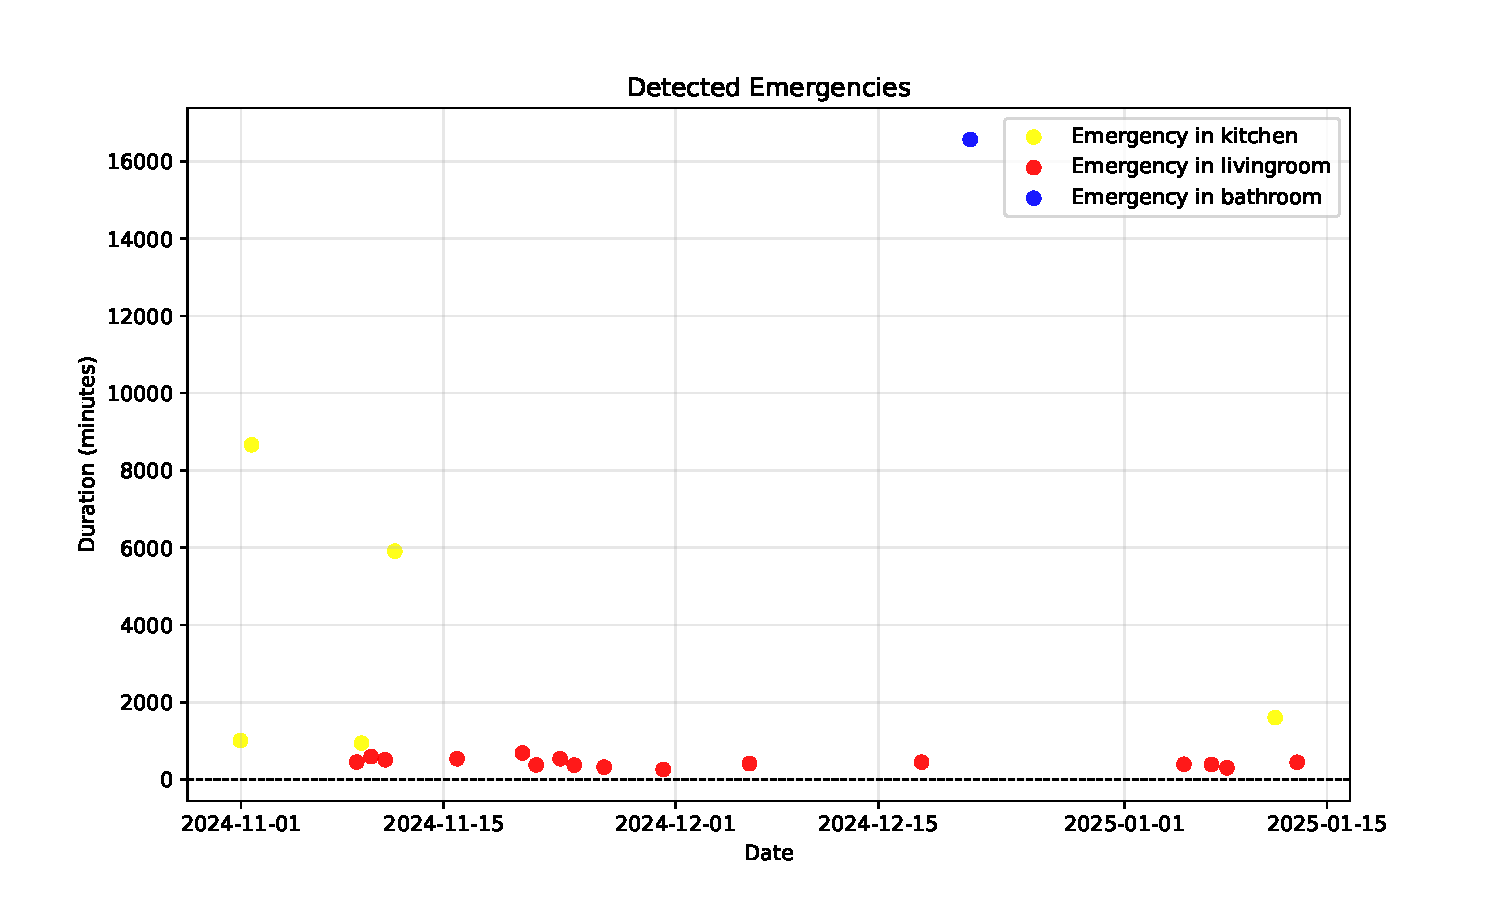
\includegraphics[width=1.15\textwidth]{detected_emergencies.pdf}
	\caption{Detected emergencies based on sensor data. Each point represents a detected emergency event.}
	\label{fig:detected_emergencies}
\end{figure}

\subsubsection{Graphs Comparing Different Weeks}
\begin{itemize}
\item Weekly means show slight variations, reflecting natural behavioral changes, such as more time in the kitchen during meals or in the living room during leisure.
\item Larger \(\sigma\) for the bathroom indicates irregular usage patterns compared to other rooms.
\item  Weekly retraining adapts to routine changes, minimizing false alarms.
\item Smaller \(\sigma\) in the kitchen room indicates consistent use patterns.

\end{itemize}

\begin{figure}[H]
	\centering
	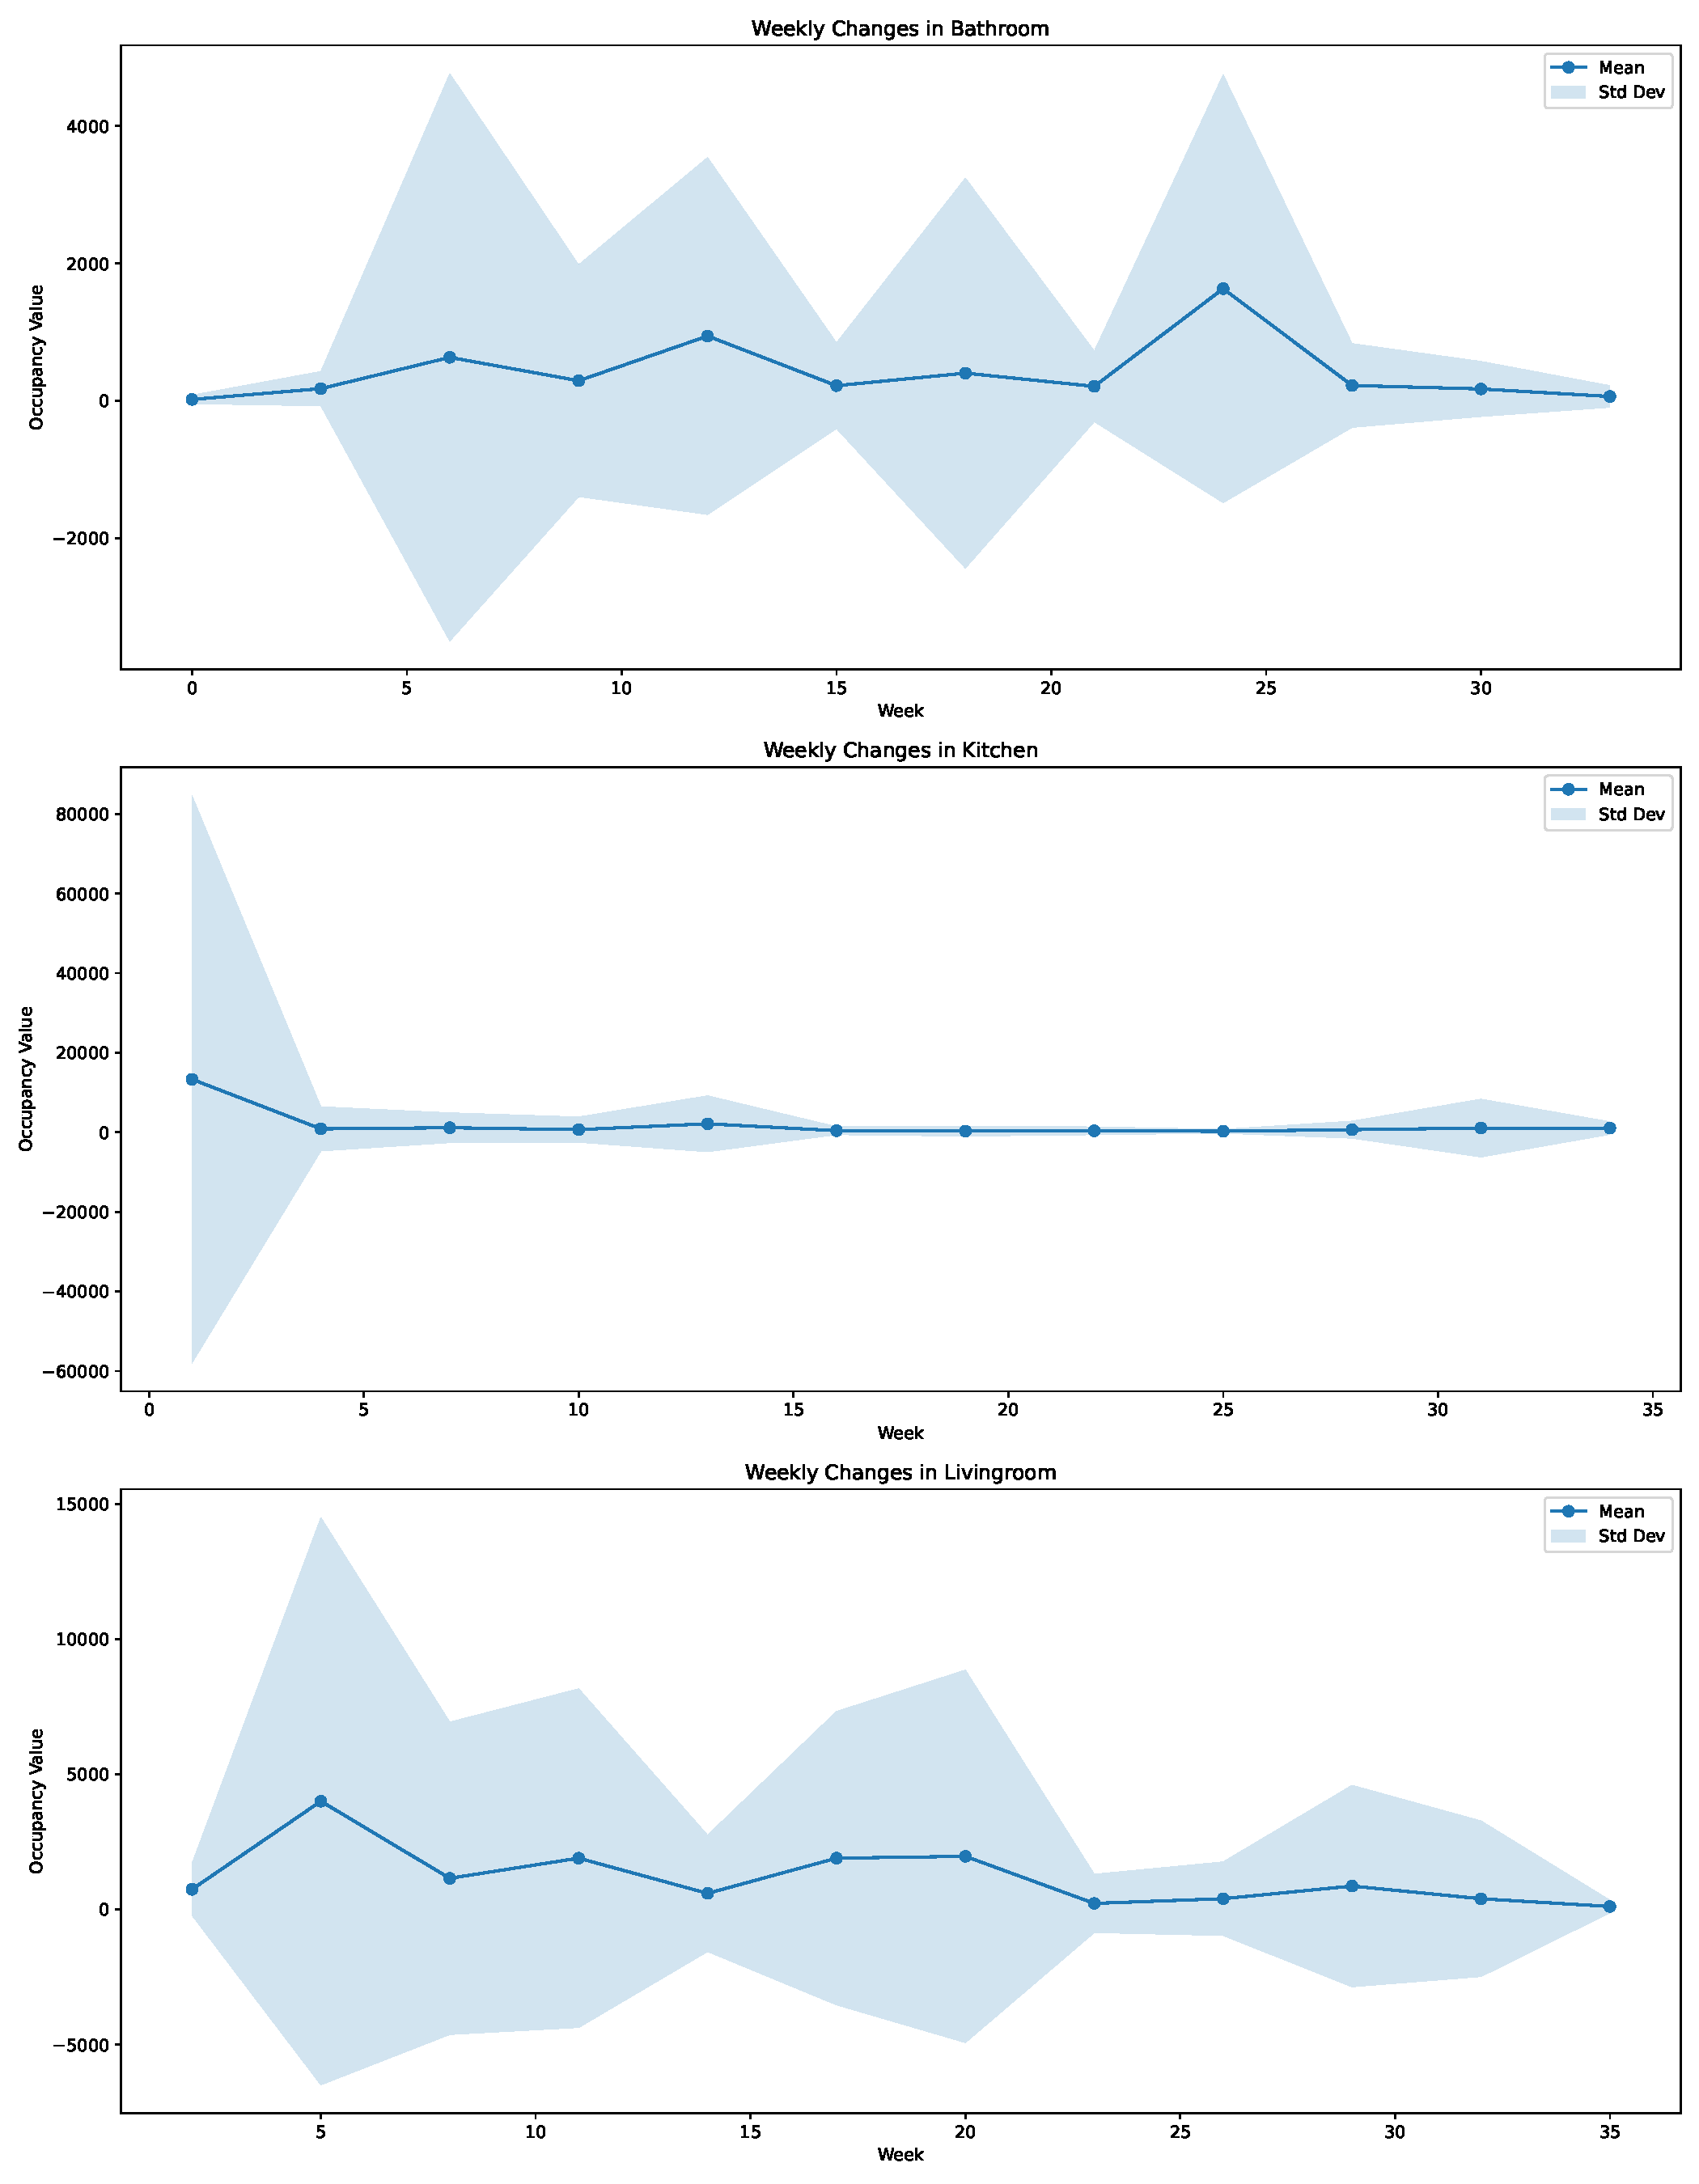
\includegraphics[width=1.15\textwidth]{weekly_changes.pdf}
	\caption{The weekly changes of the mean and std of different rooms of the apartment.}
	\label{fig:detected_emergencies}
\end{figure}

\subsection{ Use case 2: Detection of behavioral changes(3p)}

\subsubsection{Transition model training and understanding}

To train the transition model, I considered a simplified scenario where only one person is present in the apartment. If there is a change of room or a door is opened, it is interpreted as a transition. If an exit from one room is detected but no entry into another room, it is interpreted either as leaving the apartment or as falling asleep. I also try to detect wake-up times and the duration of sleep based on the first morning transitions. These detections are not always accurate because it is a simplified model that cannot distinguish between multiple residents in the apartment.

\begin{minted}[fontsize=\small]{python}
def create_transition_dataframe(df, time_threshold_seconds=3600):
	# ...
	# Determine if time difference exceeds the threshold
	if time_diff > time_threshold_seconds:
		# Determine if it's nighttime based on the hour of the previous 'leave_time'
		# Nighttime defined as 21:00 (9 PM) to 7:00 (7 AM)
		hour = previous_row['hour']
		if 21 <= hour or hour < 7:
			special_transition = 'went to sleep'
		else:
			special_transition = 'went outside'
	# ...
\end{minted}

Following code snippet shows how to detect wake-up times based on the transition model:

\begin{minted}[fontsize=\small]{python}
def detect_wake_up_times(transition_df: pd.DataFrame, transition_state: str = "went to sleep") -> pd.DataFrame:
    """
    Detects the wake-up times from a transition DataFrame.

    Filters the DataFrame for transitions where the 'from' state is "went to sleep"
    and extracts the 'leave_time' as the wake-up time.
    """
    return pd.DataFrame({
        'wake_up_time': transition_df[transition_df['from'] == transition_state]['leave_time']
    })
\end{minted}

\subsubsection{Which bahavioral changes are detected?}

The transition model analyzes motion and room transition data to detect behavioral patterns and changes in activity. It tracks movements between rooms, identifies special transitions such as sleeping or leaving the apartment, and calculates sleep duration, wake-up times, and daily room visits.

\begin{itemize}
    \item \textbf{Room Transitions:} Detect movements between rooms and identify unusual patterns.
    \item \textbf{Special Transitions:} Mark significant events such as "went to sleep" or "went outside" based on time gaps.
    \item \textbf{Daily Visits:} Count visits to critical areas like the bathroom or kitchen to monitor activity levels.
    \item \textbf{Wake-Up Times:} Identify the first activity in the morning, reflecting routine changes.
    \item \textbf{Sleep Patterns:} Analyze sleep duration and nighttime transitions for consistency or anomalies.
    \item \textbf{Transition Counts:} Summarize the frequency of movements between specific areas.
    \item \textbf{Transition Matrix:} Provide a visual representation of movement patterns between rooms.
\end{itemize}

Example comparison of two models in the period 24.11. - 1.12. 2024 (Old model) and 1.12. - 8.12.2024 (New model)

\textbf{Report Date:} 2025-12-08 23:00:00 UTC

\begin{table}[H]
\centering
\begin{tabular}{|l|l|l|}
\hline
\textbf{Day of Week} & \textbf{Old Model Sleep Time} & \textbf{New Model Sleep Time} \\ \hline
Sunday    & 1h 34m & -     \\ \hline
Monday    & 6h 32m & 8h 28m \\ \hline
Tuesday   & 1h 47m & 7h 11m \\ \hline
Wednesday & 4h 37m & 6h 54m \\ \hline
Thursday  & 6h 33m & 4h 9m  \\ \hline
Friday    & 0      & 1h 37m \\ \hline
Saturday  & 0      & 5h 58m \\ \hline
\end{tabular}
\caption{Sleep Time Summary}
\end{table}

\begin{table}[H]
\centering
\begin{tabular}{|l|l|l|}
\hline
\textbf{Day of Week} & \textbf{Old Model Bathroom Visits} & \textbf{New Model Bathroom Visits} \\ \hline
Sunday    & 29 & - \\ \hline
Monday    & 20 & 2 \\ \hline
Tuesday   & 49 & 18 \\ \hline
Wednesday & 13 & 10 \\ \hline
Thursday  & 2  & 14 \\ \hline
Friday    & -  & 73 \\ \hline
Saturday  & -  & 38 \\ \hline
\end{tabular}
\caption{Daily Visits to Bathroom}
\end{table}


\begin{table}[H]
\centering
\begin{tabular}{|l|l|l|}
\hline
\textbf{Day of Week} & \textbf{Old Model Kitchen Visits} & \textbf{New Model Kitchen Visits} \\ \hline
Sunday    & 34 & - \\ \hline
Monday    & 23 & 1 \\ \hline
Tuesday   & 55 & - \\ \hline
Wednesday & 13 & 8 \\ \hline
Thursday  & 9  & 23 \\ \hline
Friday    & 11 & 80 \\ \hline
Saturday  & 23 & 41 \\ \hline
\end{tabular}
\caption{Daily Visits to Kitchen}
\end{table}


\begin{table}[H]
\centering
\begin{tabular}{|l|l|l|}
\hline
\textbf{Day of Week} & \textbf{Old Model Wake-Up Time} & \textbf{New Model Wake-Up Time} \\ \hline
Sunday    & 05:26:02 & 23:05:45 \\ \hline
Monday    & 17:29:48 & 04:23:16 \\ \hline
Tuesday   & 01:47:15 & 07:56:43 \\ \hline
Wednesday & 01:54:12 & 07:11:50 \\ \hline
Thursday  & 02:29:05 & 06:01:07 \\ \hline
Friday    & 08:32:14 & 07:22:04 \\ \hline
Saturday  & 05:42:15 & 04:24:58 \\ \hline
\end{tabular}
\caption{Wake-Up Times}
\end{table}


\begin{table}[H]
\centering
\begin{tabular}{|l|l|l|}
\hline
\textbf{Day of Week} & \textbf{Old Model Went-To-Sleep Time} & \textbf{New Model Went-To-Sleep Time} \\ \hline
Sunday    & 22:25:35 & 22:12:10 \\ \hline
Monday    & 16:50:49 & 23:08:19 \\ \hline
Tuesday   & 23:32:08 & 04:23:16 \\ \hline
Wednesday & 00:41:32 & 23:28:33 \\ \hline
Thursday  & 01:54:12 & 00:14:02 \\ \hline
Friday    & 07:04:22 & 06:14:26 \\ \hline
Saturday  & 22:38:24 & 01:14:20 \\ \hline
\end{tabular}
\caption{Went-To-Sleep Times}
\end{table}


\begin{figure}[H]
	\centering
	\begin{minipage}{0.45\textwidth}
		\centering
		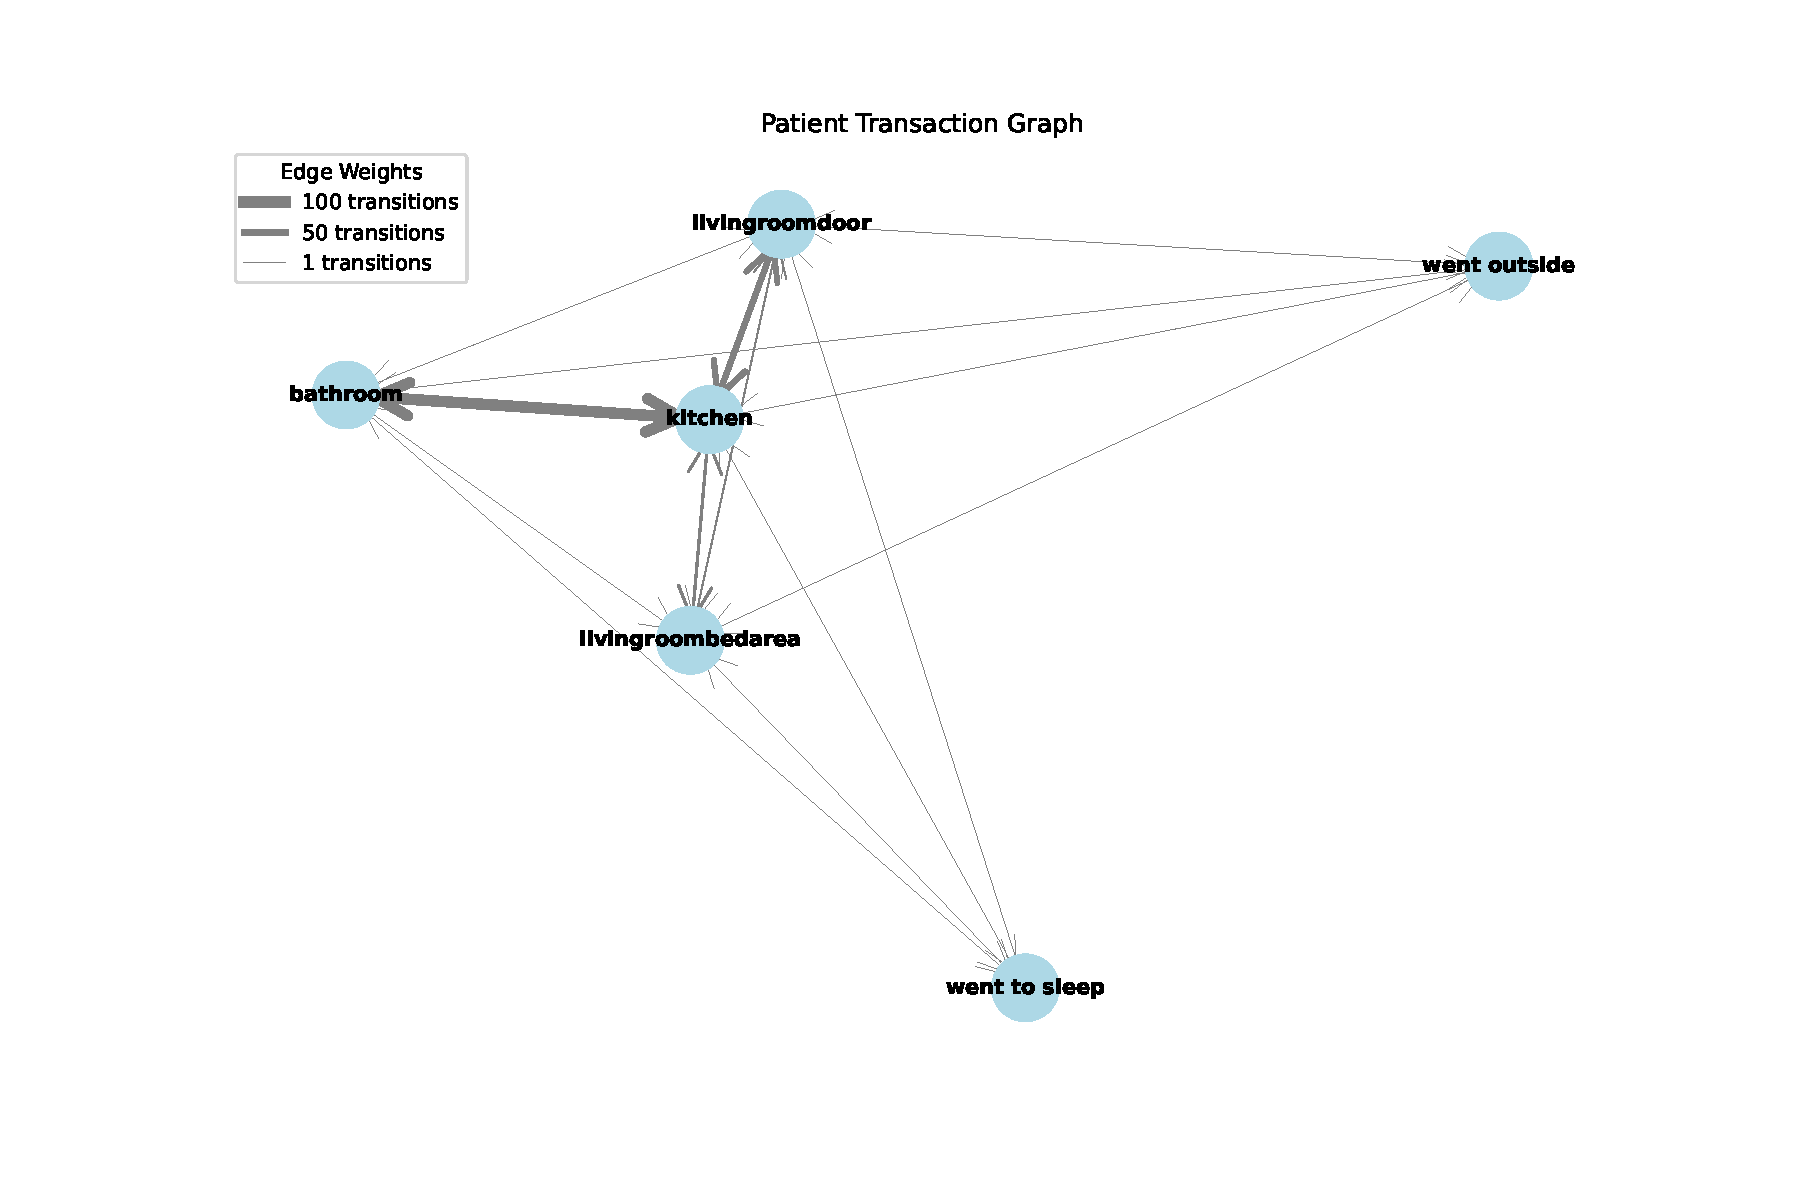
\includegraphics[width=\textwidth]{biderictional_model1.pdf}
		\caption{Bidirectional Graph Of Transitions (24.11.- 1.12.2024)}
		\label{fig:model1}
	\end{minipage}\hspace{0.04\textwidth}
	\begin{minipage}{0.45\textwidth}
		\centering
		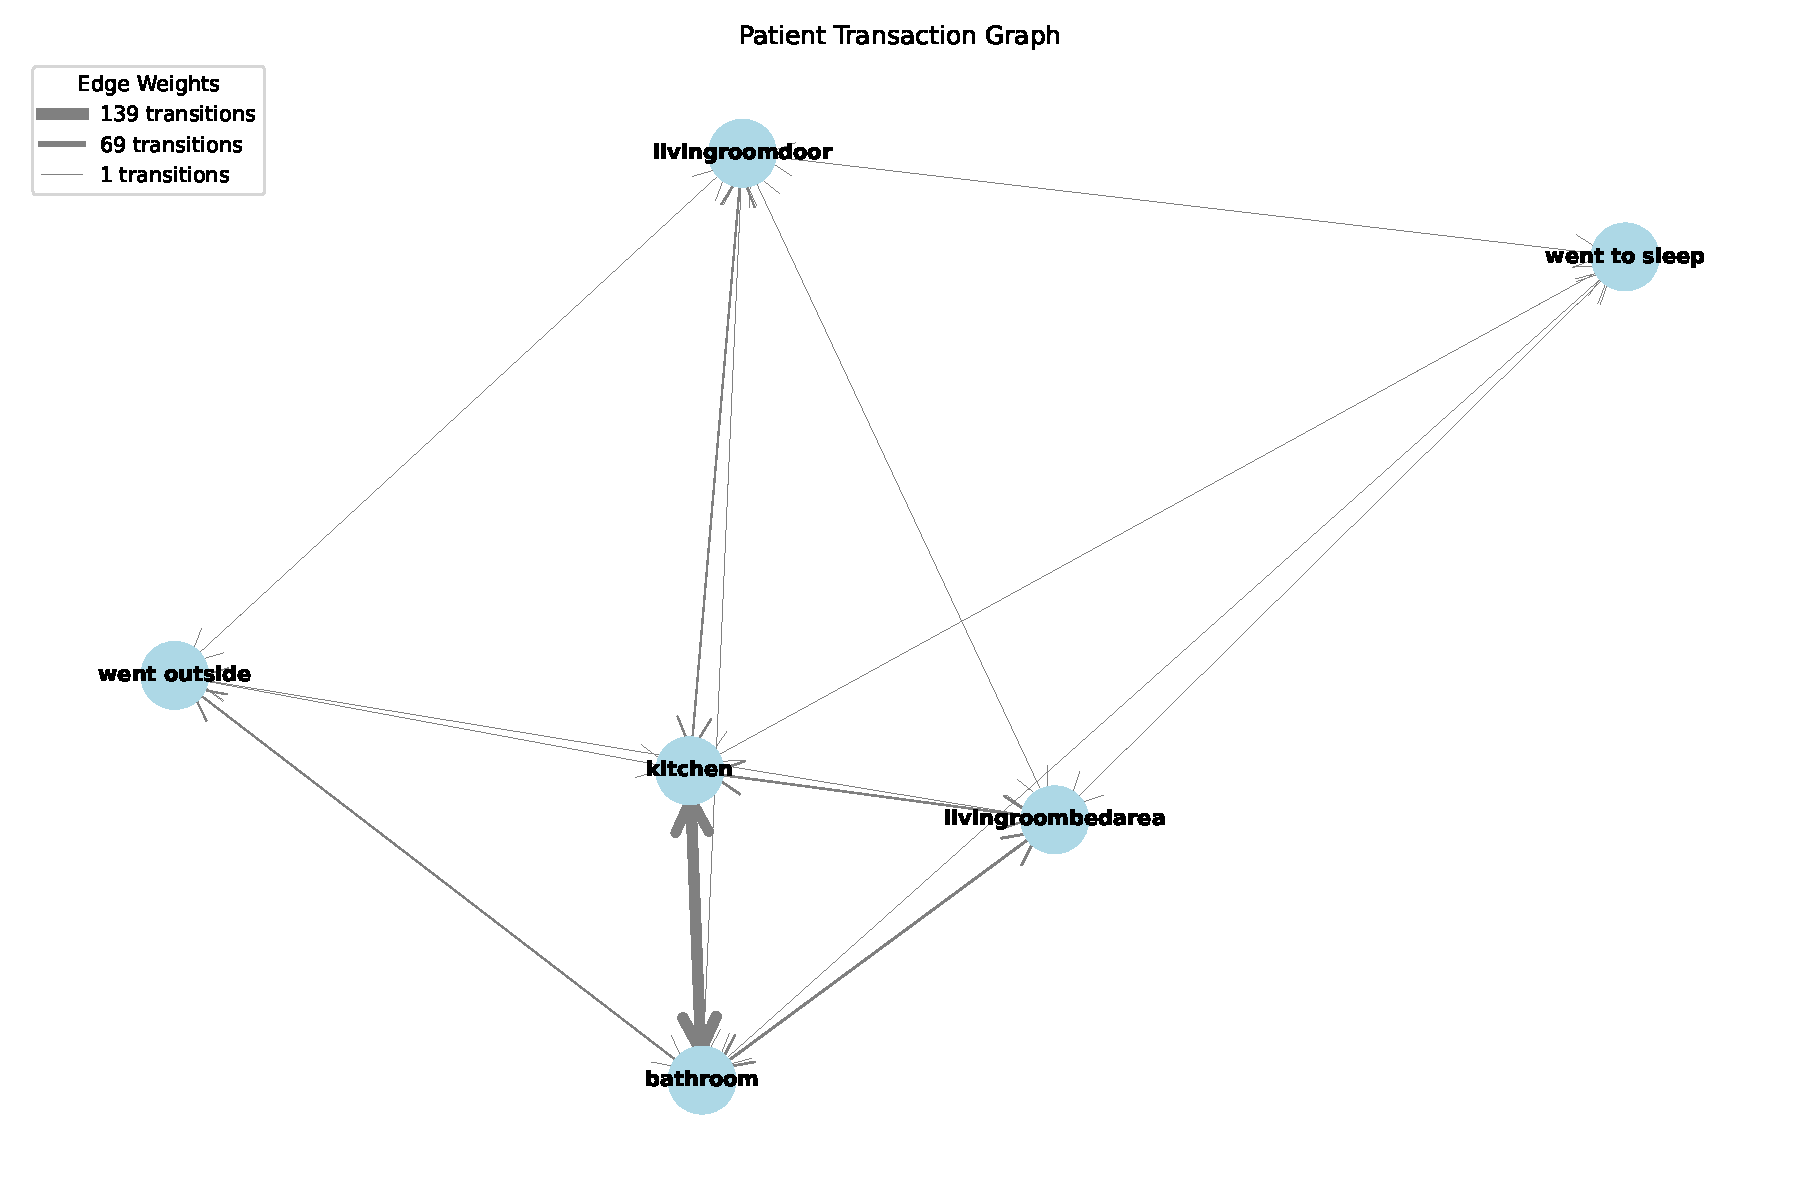
\includegraphics[width=\textwidth]{biderictional_model2.pdf}
		\caption{Bidirectional Graph Of Transitions (1.12.- 8.12.2024)}
		\label{fig:model2}
	\end{minipage}
\end{figure}

\begin{figure}[H]
	\centering
	\begin{minipage}{0.45\textwidth}
		\centering 
		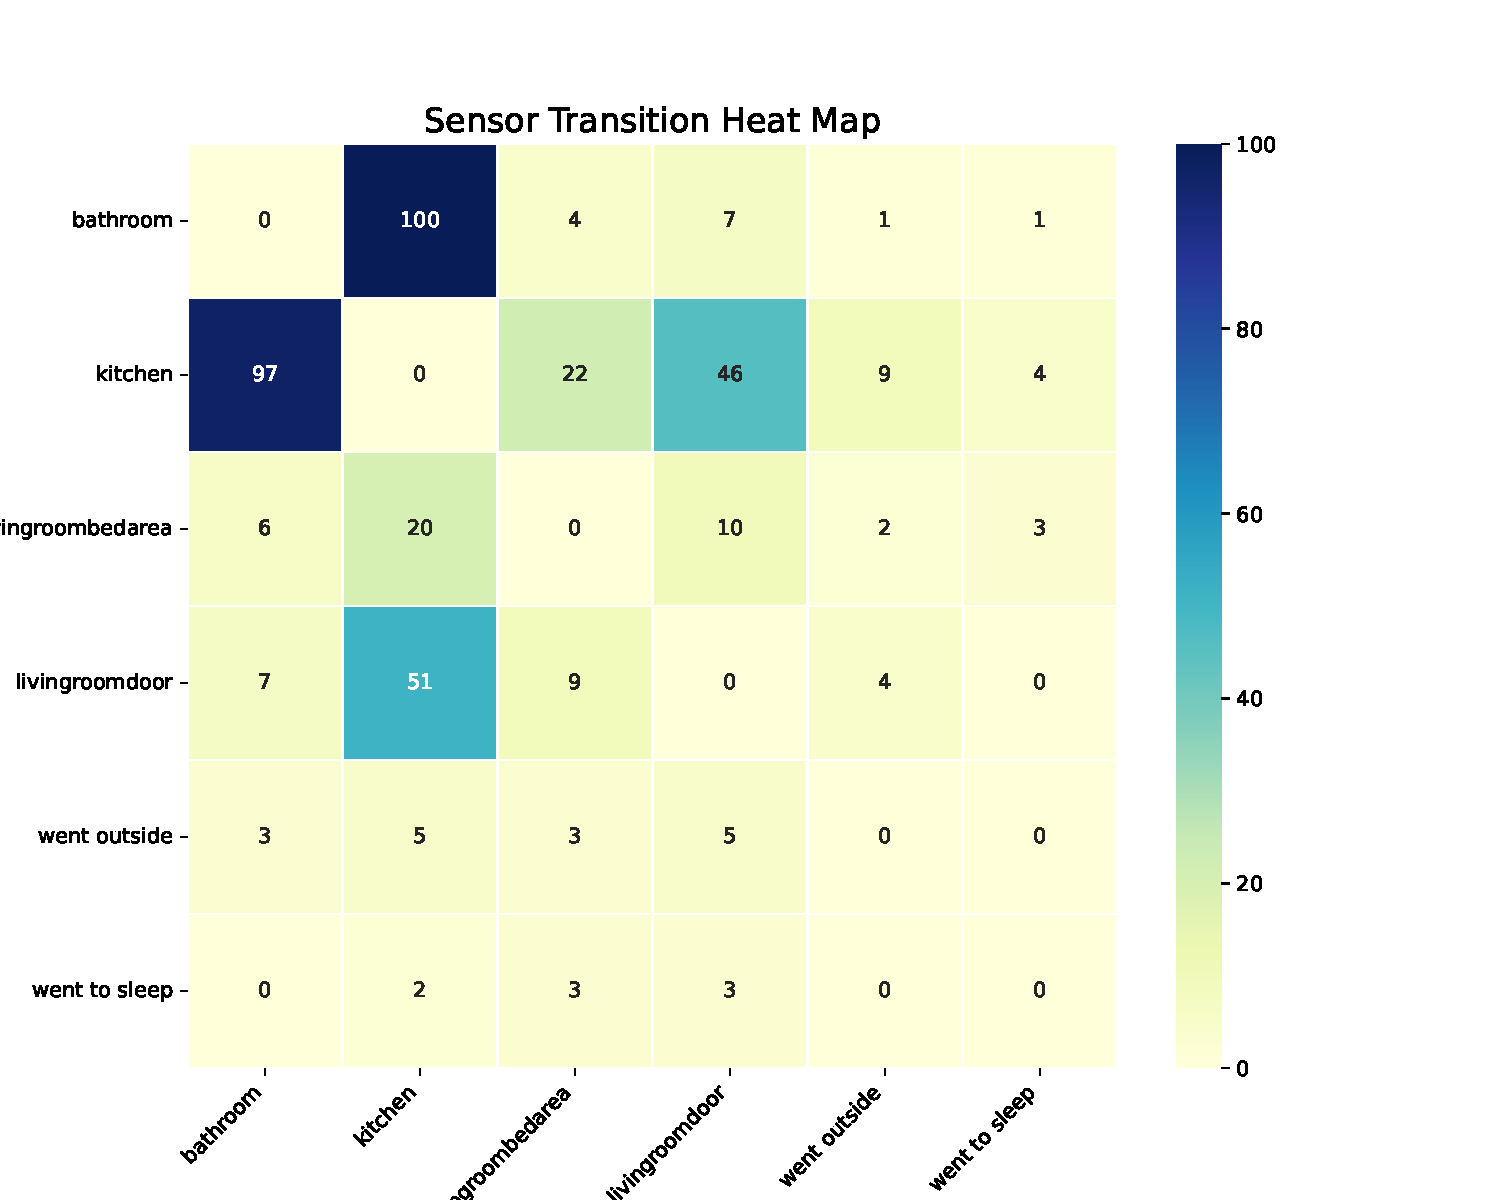
\includegraphics[width=\textwidth]{heatmap1.pdf}
		\caption{Heatmap of Weekly Transitions (24.11.- 1.12.2024)}
		\label{fig:heatmap1}
	\end{minipage}\hspace{0.04\textwidth}
	\begin{minipage}{0.45\textwidth}
		\centering
		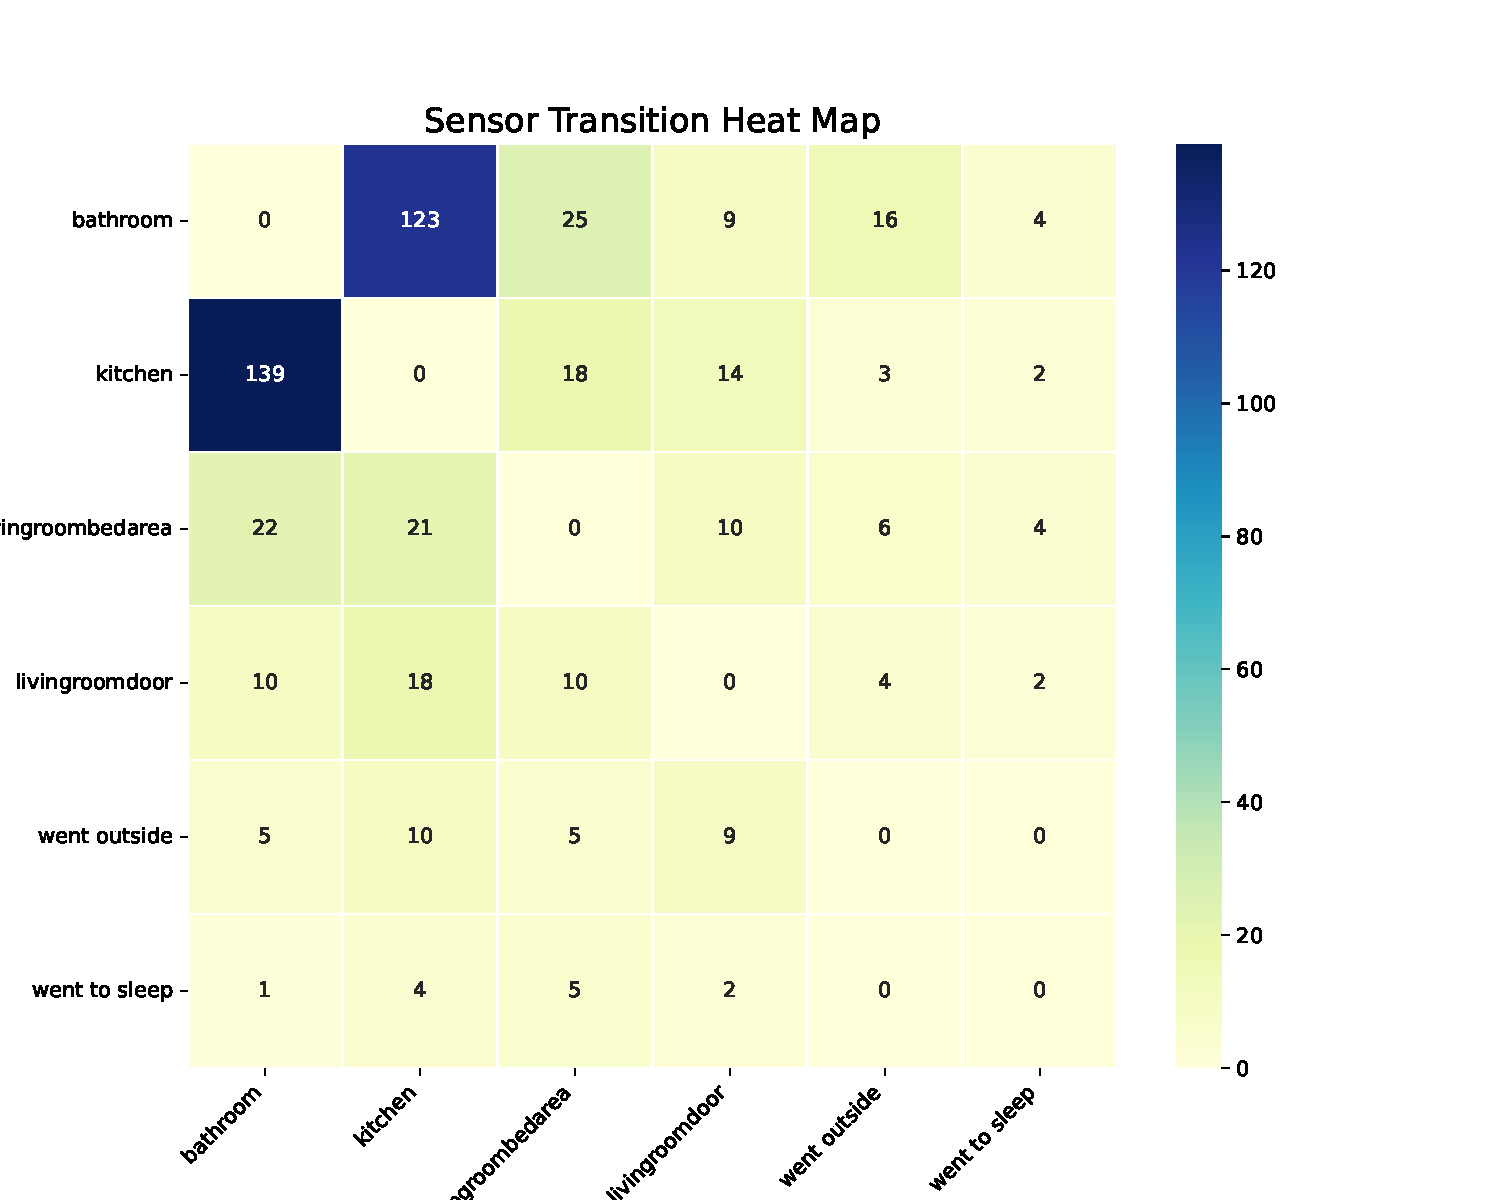
\includegraphics[width=\textwidth]{heatmap2.pdf}
		\caption{Heatmap of Weekly Transitions (1.12.- 8.12.2024)}
		\label{fig:heatmap2}
	\end{minipage}
\end{figure}

\begin{figure}[H]
	\centering
	\begin{minipage}{0.45\textwidth}
		\centering
		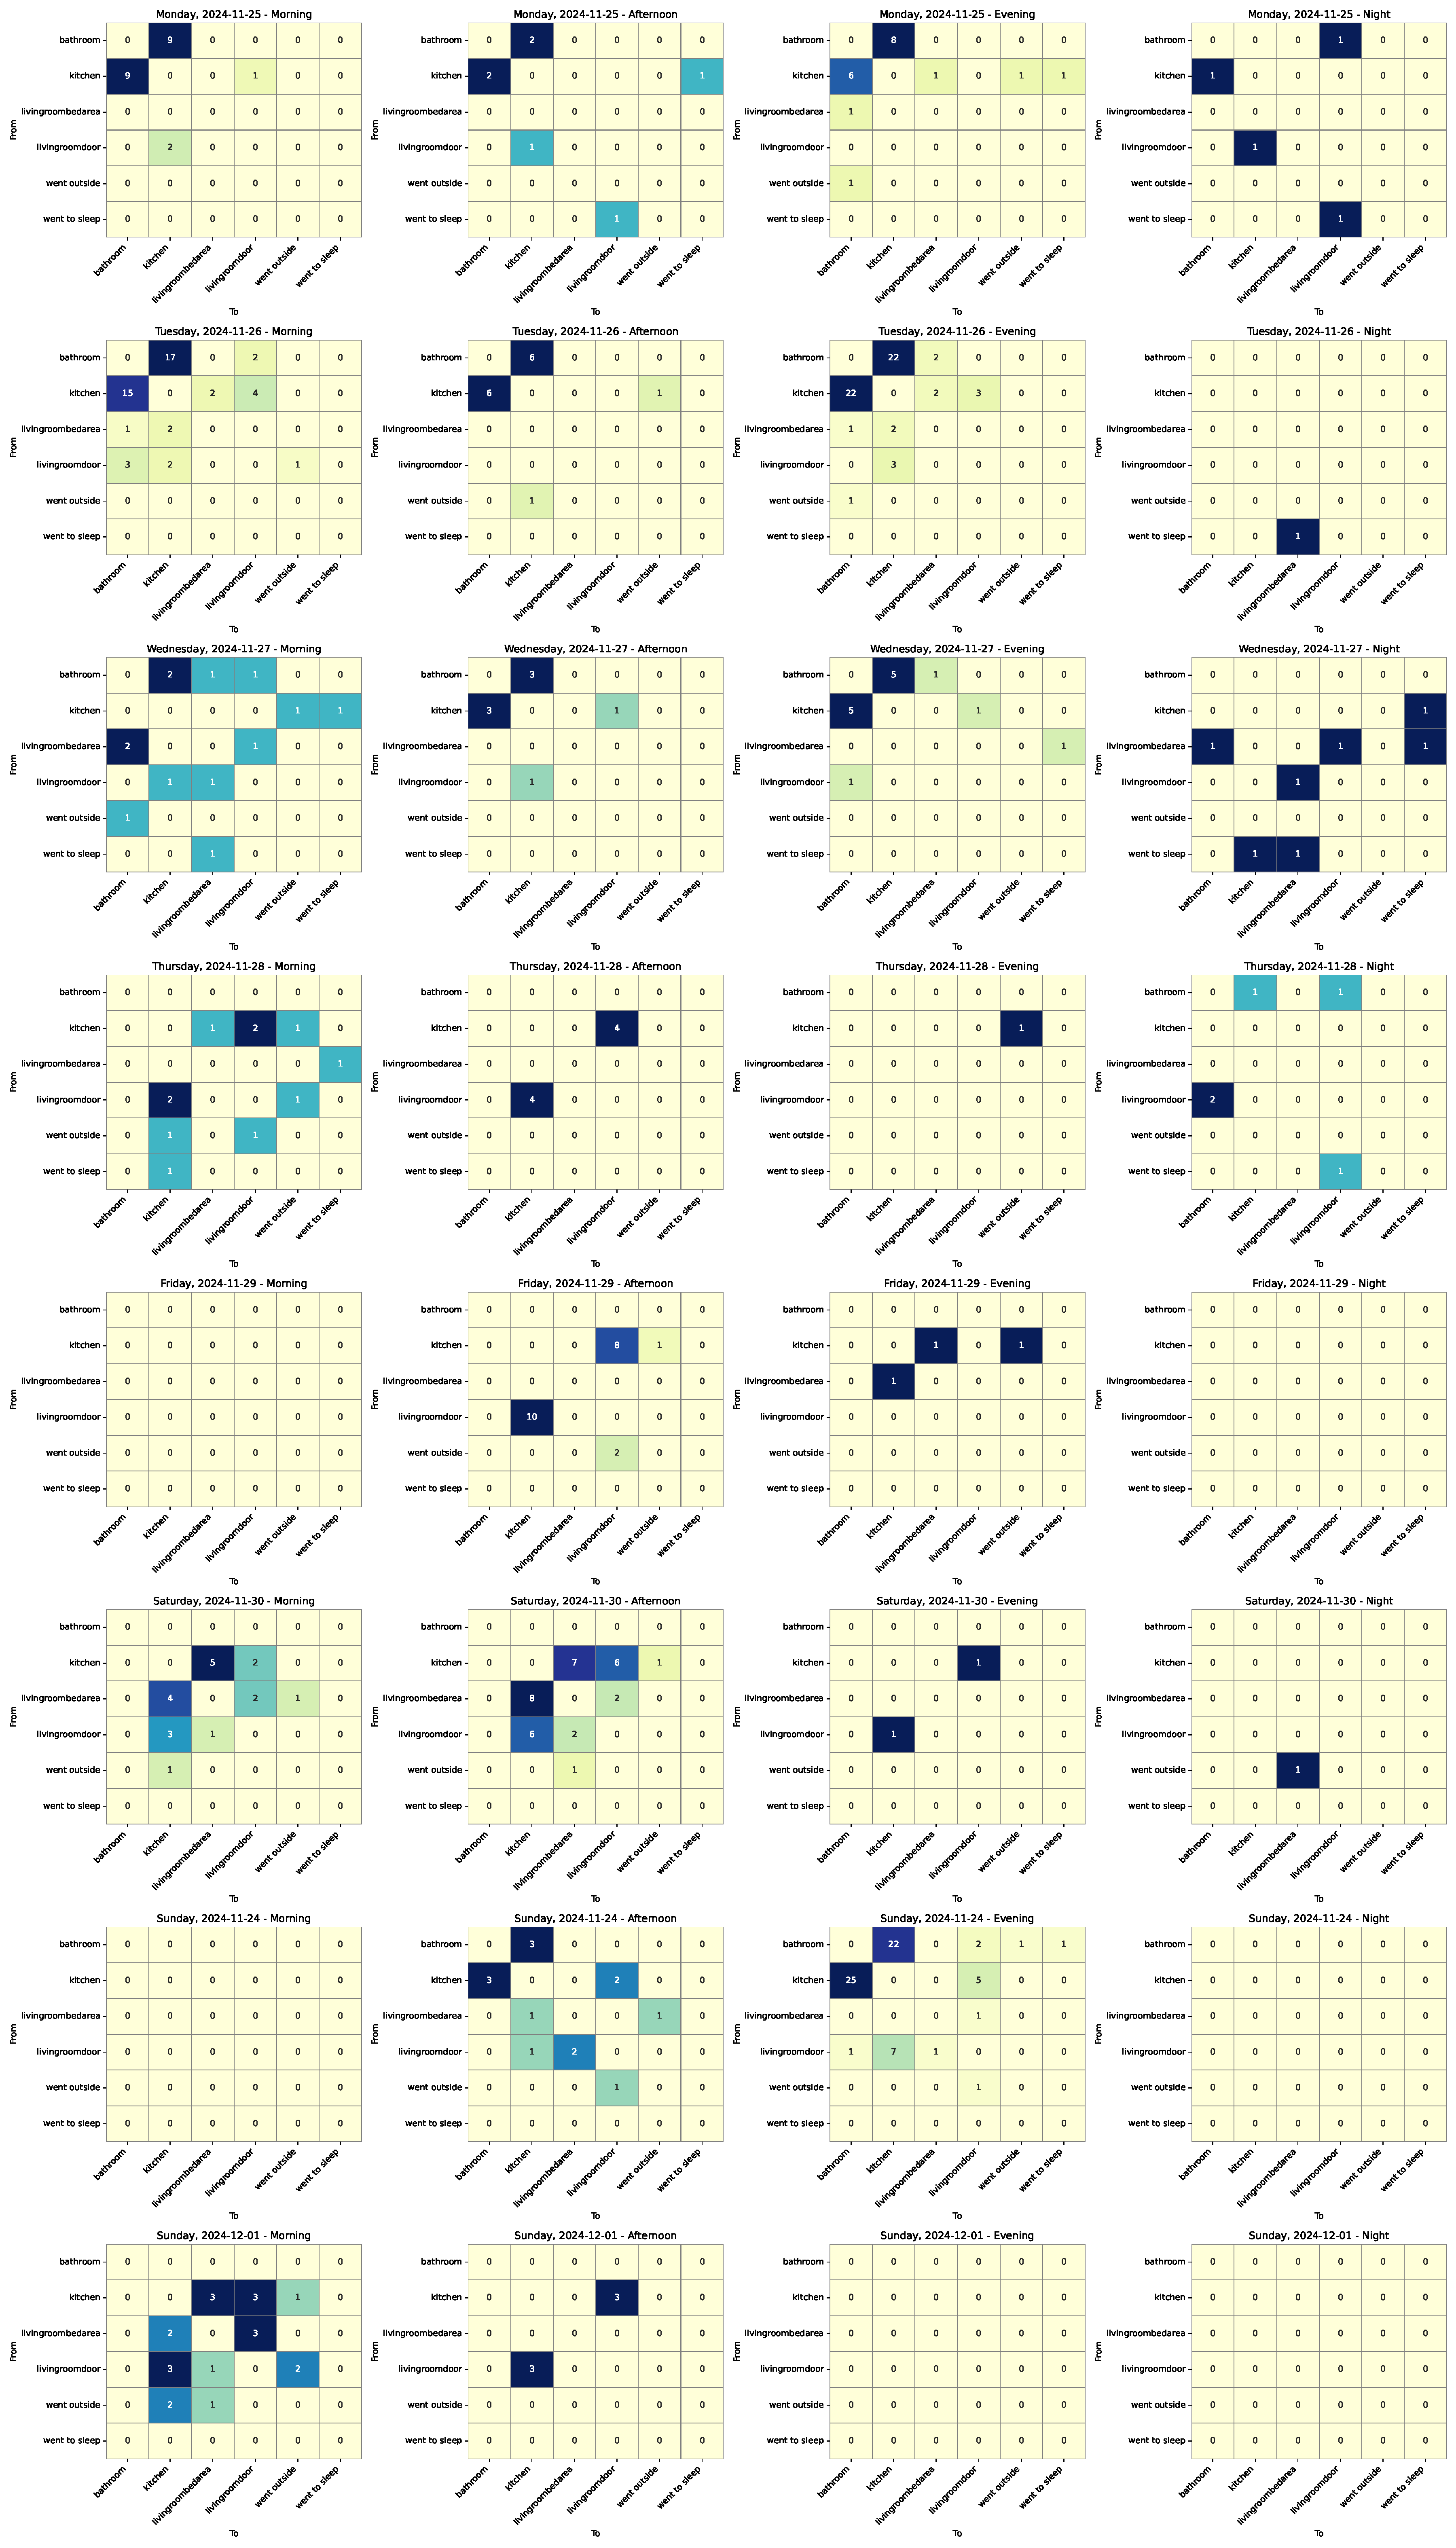
\includegraphics[width=\textwidth]{heatmap_days1.pdf}
		\caption{Heatmap of Daily Transitions (24.11.- 1.12.2024)}
		\label{fig:heatmap1}
	\end{minipage}\hspace{0.04\textwidth}
	\begin{minipage}{0.45\textwidth}
		\centering
		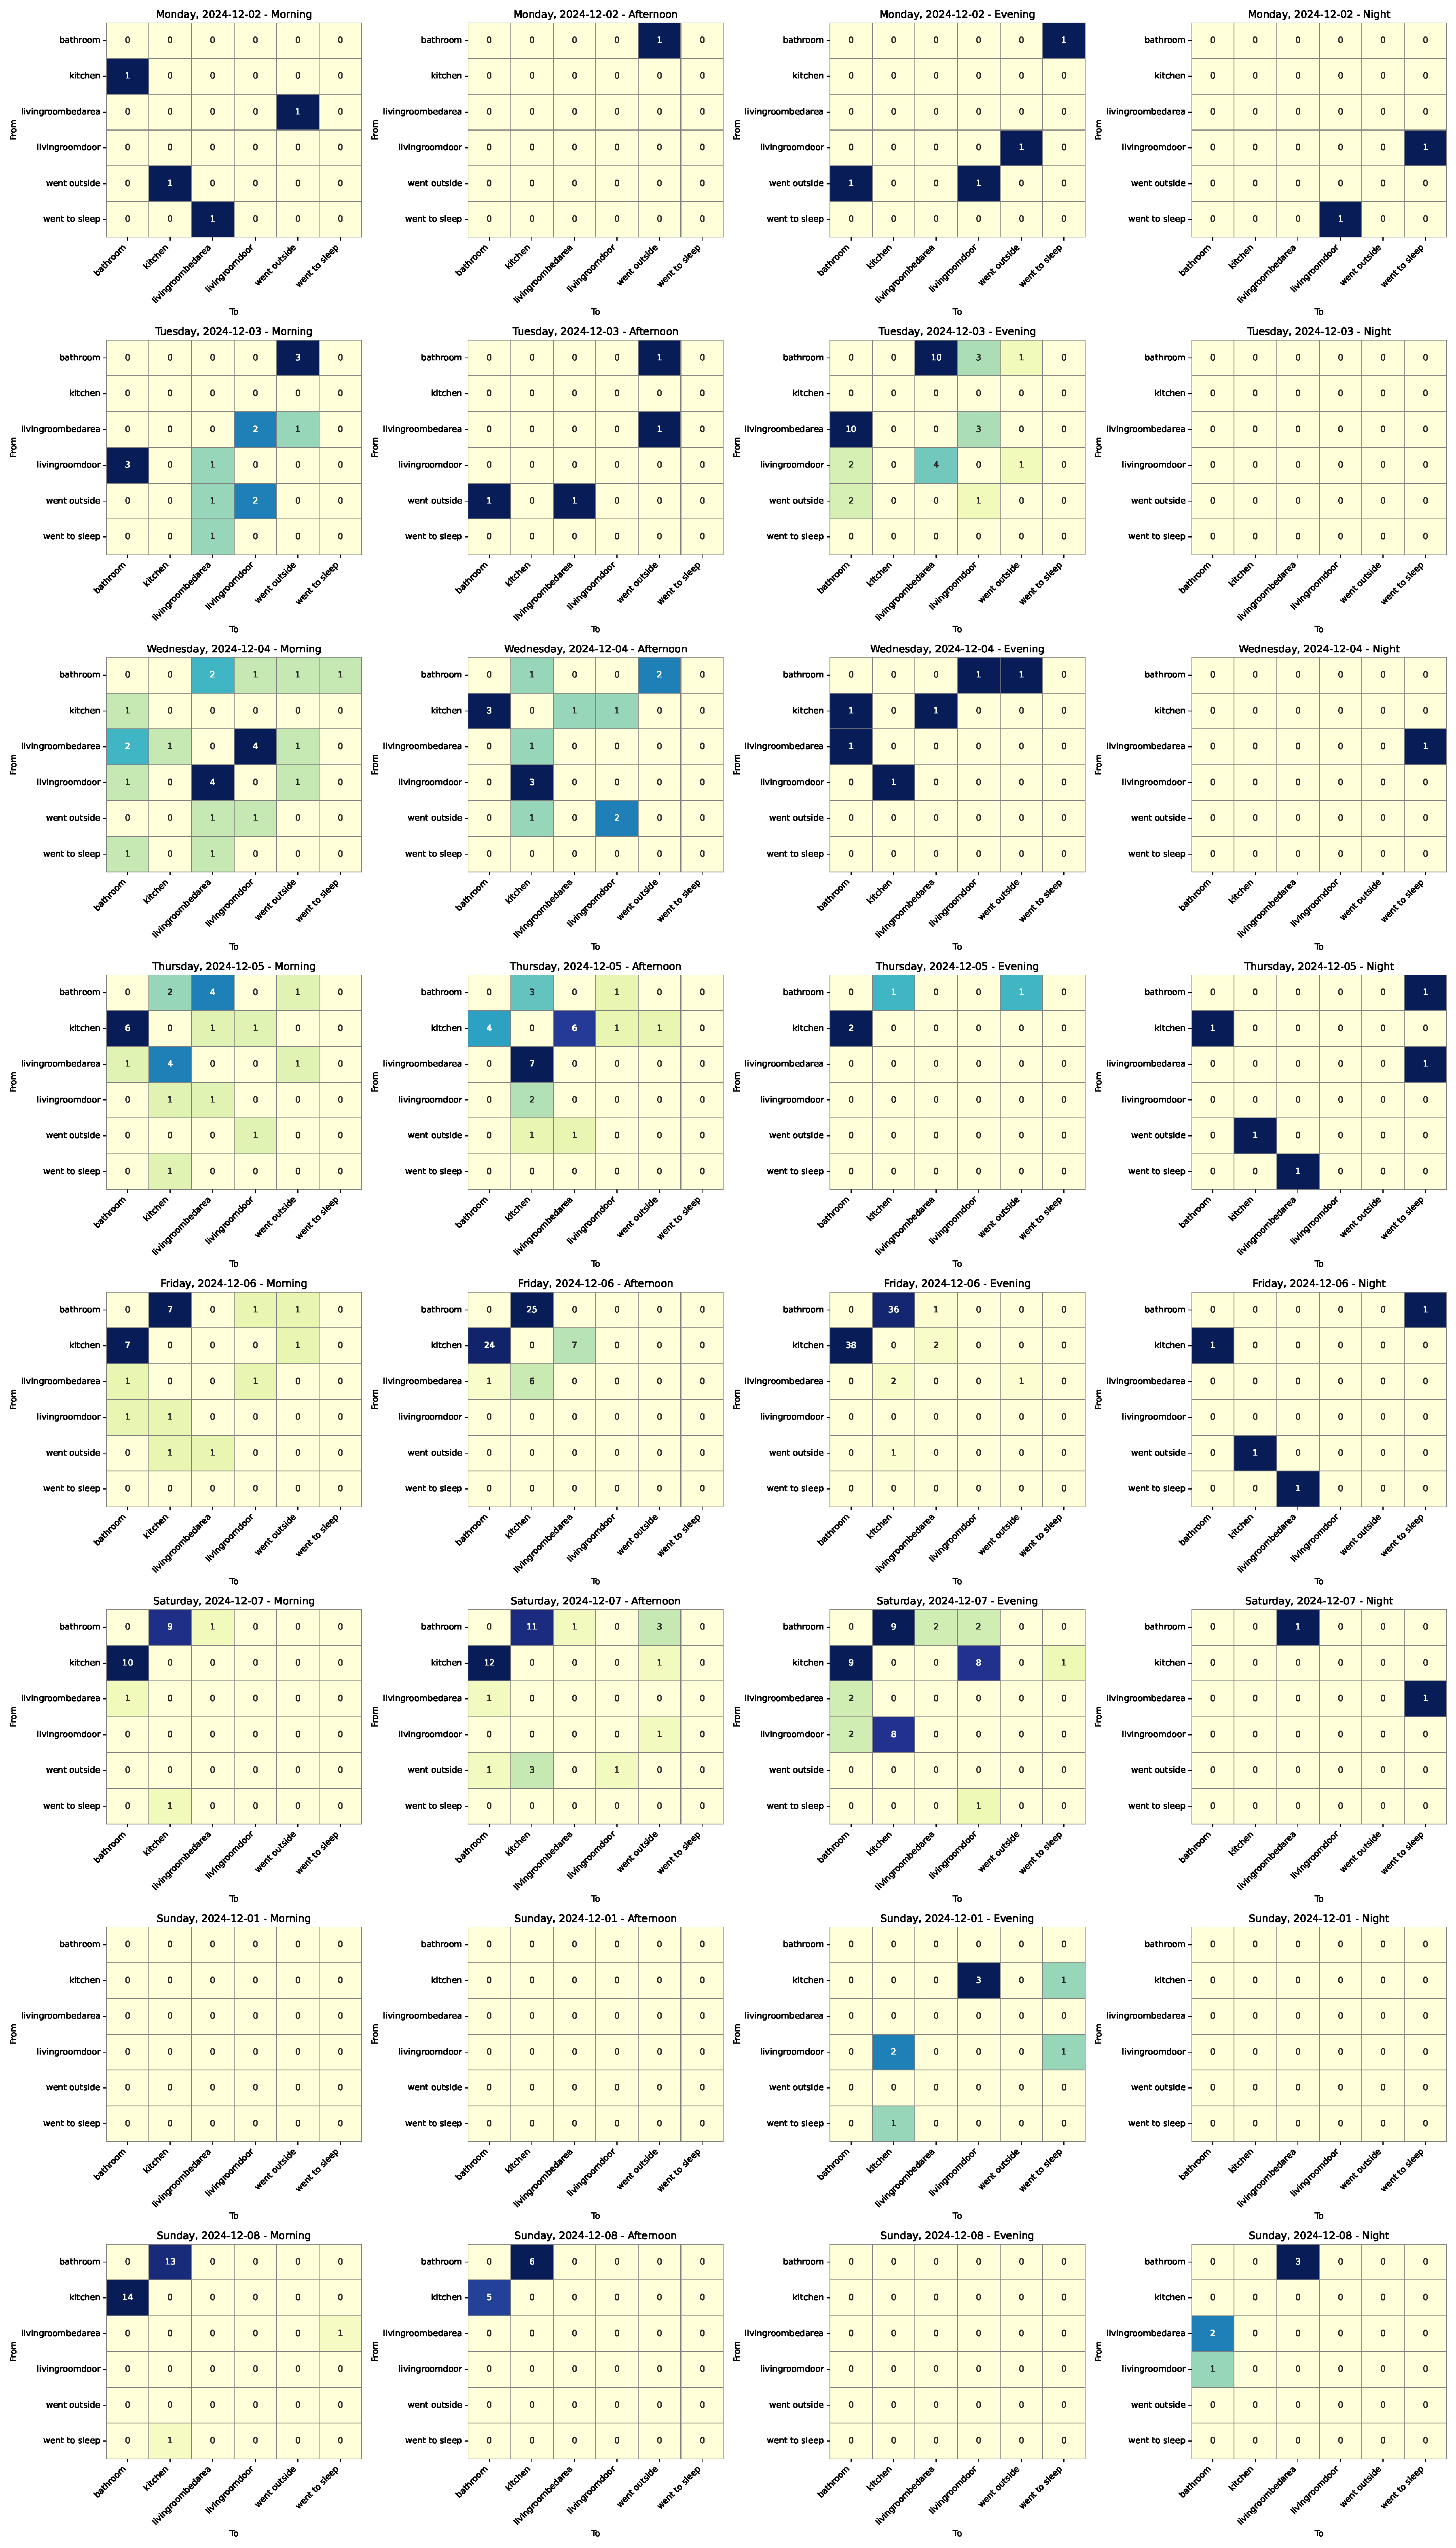
\includegraphics[width=\textwidth]{heatmap_days2.pdf}
		\caption{Heatmap of Daily Transitions (1.12.- 8.12.2024)}
		\label{fig:heatmap2}
	\end{minipage}
\end{figure}

\begin{figure}[H]
	\centering
	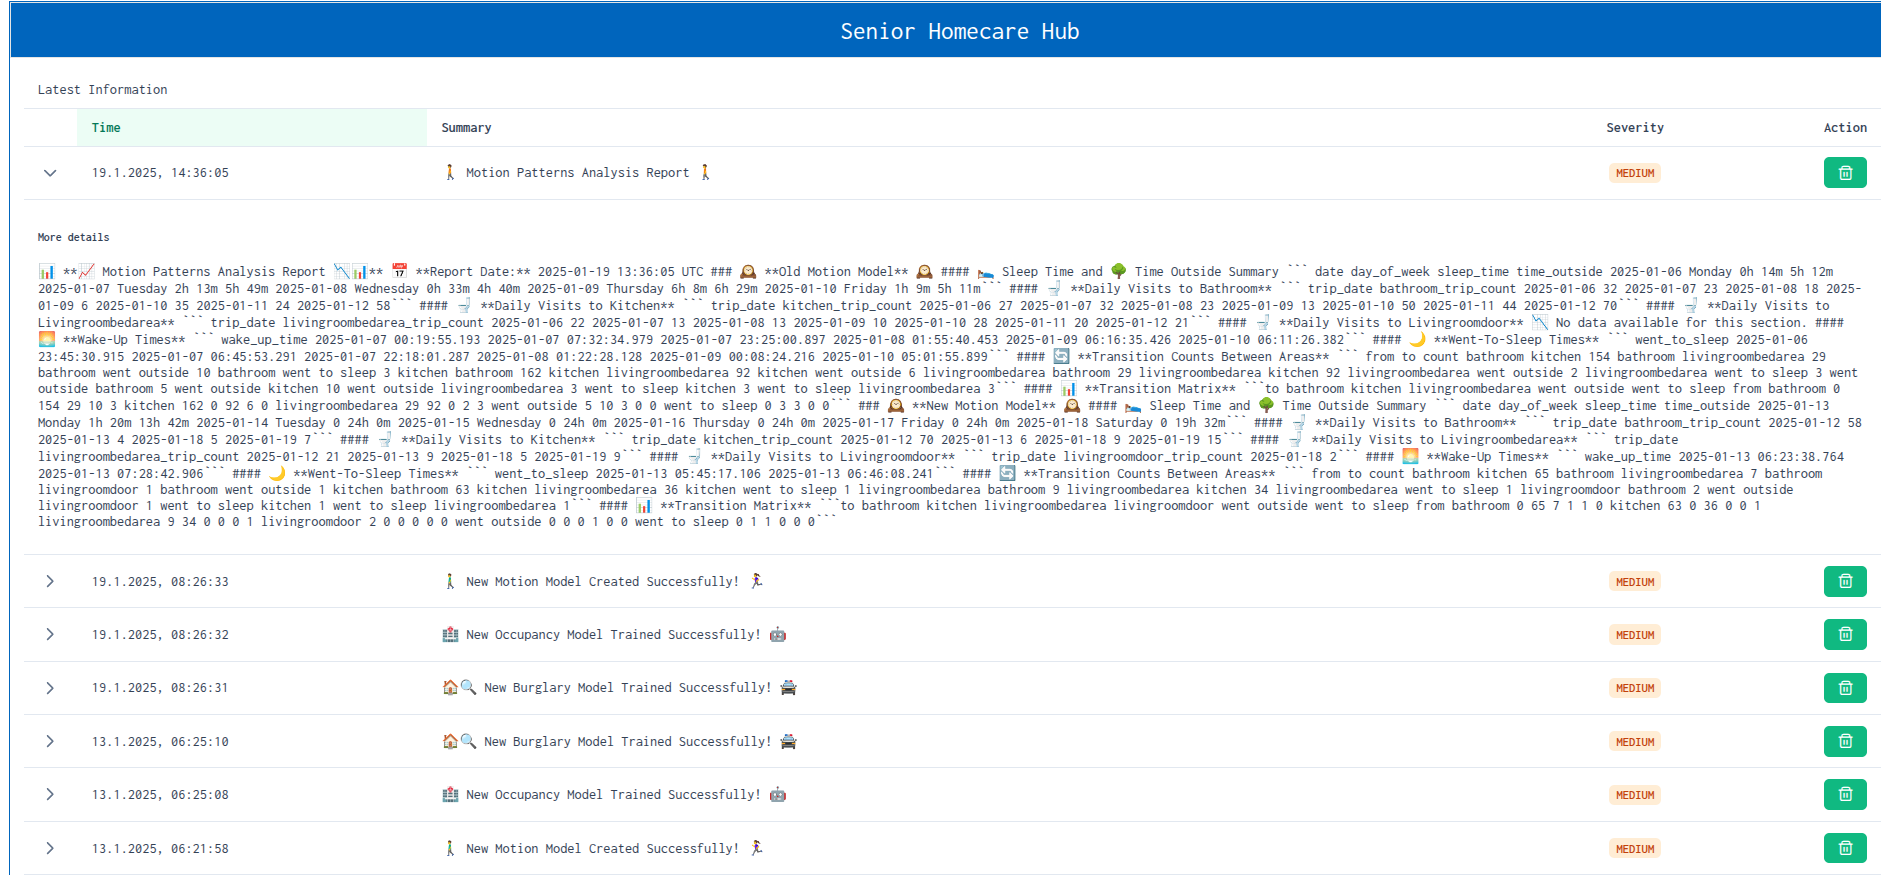
\includegraphics[width=1.1\textwidth]{homecare-hub01.png}
	\caption{The communication with the homecare-hub.}
	\label{fig:hub}
\end{figure}

\begin{itemize}
	\item \textbf{Limitations of the Model:} The model cannot accurately capture movements involving multiple persons or more complex behavioral changes. It is designed for simpler, single-occupant scenarios. It also might misinterpet the leaving of the apartment and falling asleep.
	\item \textbf{Modeling Approach Selection:} The approach for detecting behavioral changes was chosen for its simplicity and effectiveness. By comparing models from the last two weeks, caregivers can easily identify significant changes in behavior.
	\item \textbf{Differentiating Information and To-Do Messages:} The differentiation between an "information" message and a "to-do" message is based on the modeling approach. The highest emergency is only for burglary and patient emergency event, during behavioral analysis I dont do any emergency detection.
	\item \textbf{Communication with Visualization Component:} Information is communicated to the visualization component as shown in the provided image, ensuring that relevant data is displayed (unfortunaly not so clearly).
	\item \textbf{Severity Calculation:} The severity of alerts is not dynamically calculated; it is assigned a fixed value based on predefined criteria.
	\item \textbf{Emergency Detection Capability:} Yes, the modeling approach (The emergency model) is capable of determining emergencies, as illustrated in the graph above. However, the motion and behaviour model is not designed for detecting emergiences, rather then for showing the weekly trends to the caregivers
\end{itemize}


\subsection{ Use case 3: Burglary Detection (4p)}

My own use case for the homecare hub involved burglary detection. For detection, I used Isolation Forest, which is capable of detecting anomalies in data. In this case, I used data on transitions between rooms (with times of the transitions). I chose this model because I concluded that it would be easier to perform such anomaly detection for an apartment with multiple occupants. I used Isolation Forest because it can detect anomalies in data that are mutually independent.

\begin{minted}[fontsize=\small]{python}
class BurglaryDetector:
    def __init__(self, contamination='auto', random_state=42, model_type: str = 'burglary'):
        """
        Initializes the BurglaryDetector with specified Isolation Forest parameters.

        Parameters:
        - contamination: float, 'auto' or float, the proportion of anomalies in the data set.
        - random_state: int, random seed for reproducibility.
        - model_type: str, identifier for the model type (used in MinIO storage).
        """
        self.contamination = contamination
        self.random_state = random_state
        self.model = None
        self.preprocessor = None
        self.feature_columns = None
        self.model_type = model_type
    # ...
    def train(self, df: pd.DataFrame):
        """
        Trains the Isolation Forest model on the provided DataFrame.

        Parameters:
        - df: pandas DataFrame with columns ['from', 'to', 'leave_time', 'enter_time'].
        """
        # Feature engineering
        df_features, _ = self._feature_engineering(df.copy())
        # Separate features and prepare the pipeline
        X = df_features.copy()
        # Initialize Isolation Forest within a Pipeline
        self.model = Pipeline(steps=[
            ('preprocessor', self.preprocessor),
            ('classifier', IsolationForest(
                n_estimators=100,
                contamination=self.contamination,
                random_state=self.random_state
            ))
        ])
        # Fit the model
        self.model.fit(X)
        # Store feature columns after preprocessing for reference
        self.feature_columns = self.model.named_steps['preprocessor'].get_feature_names_out()
    #...
    def detect_burglary(start_hours=2, interval_hours=2, time_threshold_seconds=1800):
        """
        Detects potential burglaries based on motion data and generates an appropriate message.
        Parameters:
        - start_hours (int): Starting hours for motion data analysis.
        - interval_hours (int): Number of hours over which to aggregate motion data (e.g., 24 for daily).
        - time_threshold_seconds (int): Threshold in seconds to filter motion durations (e.g., 1800 for 30 minutes).

        Returns:
        - Tuple[Optional[bool], Optional[str]]: A tuple containing:
            - is_burglary (bool): Indicates whether any anomalies (potential burglaries) were detected.
            - message (str): A formatted message detailing the detection results.
        """
        detector = BurglaryDetector(contamination=0.01, model_type='burglary')
        detector.load_model(version=1)
        motion_model = train_motion_model(
            start_hours=start_hours, 
            interval_hours=interval_hours, 
            time_threshold_seconds=time_threshold_seconds)
        detection = detector.detect(motion_model)
        message = create_burglary_message(detection[0], detection[1])
        return detection[1], message
\end{minted}

\subsubsection{Algorithm Parameters}
\begin{itemize}[noitemsep, topsep=0pt]
    \item \textbf{Number of Trees ($n\_estimators$)}: Determines the number of decision trees in the forest. A larger number improves accuracy but increases computation time.
    \item \textbf{Contamination ($contamination$)}: Proportion of the dataset expected to be anomalies. This parameter affects the threshold for classifying anomalies.
    \item \textbf{Random State ($random\_state$)}: Ensures reproducibility by setting a fixed seed for random number generation.
    \item \textbf{Subsample Size}: Number of samples used to construct each tree. Smaller subsamples increase randomness and reduce computation.
\end{itemize}

This \texttt{detect\_burglary} function performs the following steps:
\begin{enumerate}
    \item Initializes the \texttt{BurglaryDetector} with specified parameters.
    \item Loads the latest trained model from MinIO.
    \item Trains the motion model using the provided parameters.
    \item Detects anomalies in the trained motion model.
    \item Generates a formatted message based on the detection results.
\end{enumerate}

\begin{figure}[H]
	\centering
	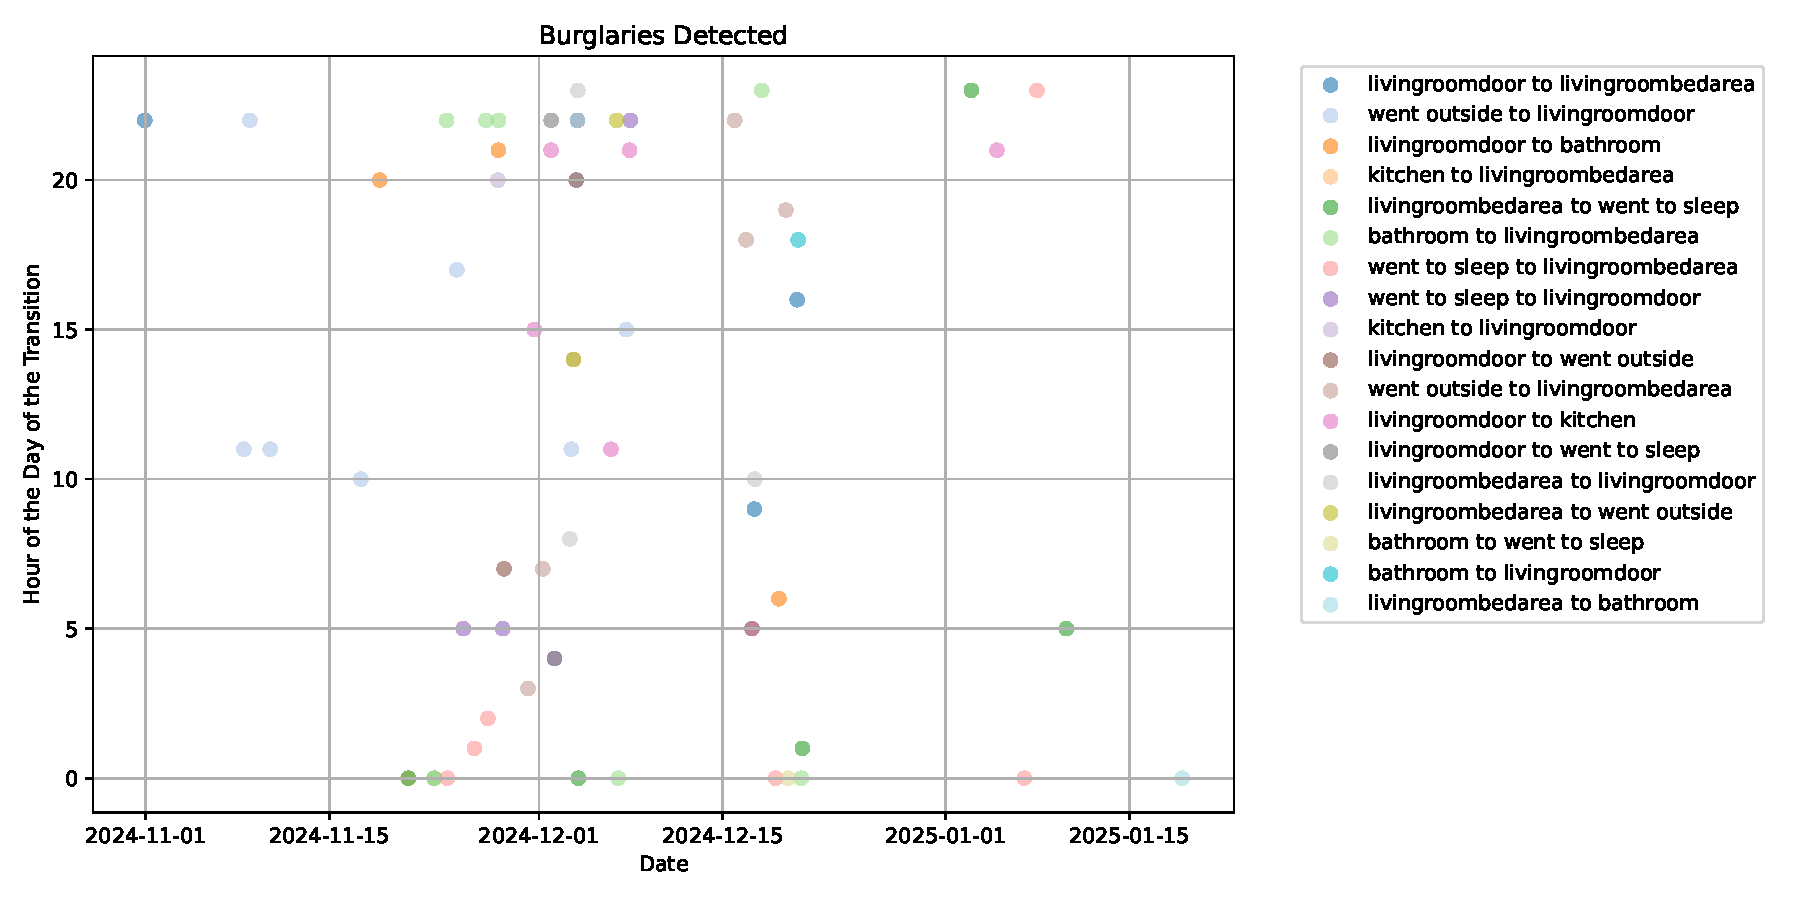
\includegraphics[width=1.1\textwidth]{burglaries_detected.pdf}
	\caption{The detected burglaries based on transition data. Each point represents a detected burglary event.}
	\label{fig:hub}
\end{figure}

\begin{figure}[H]
	\centering
	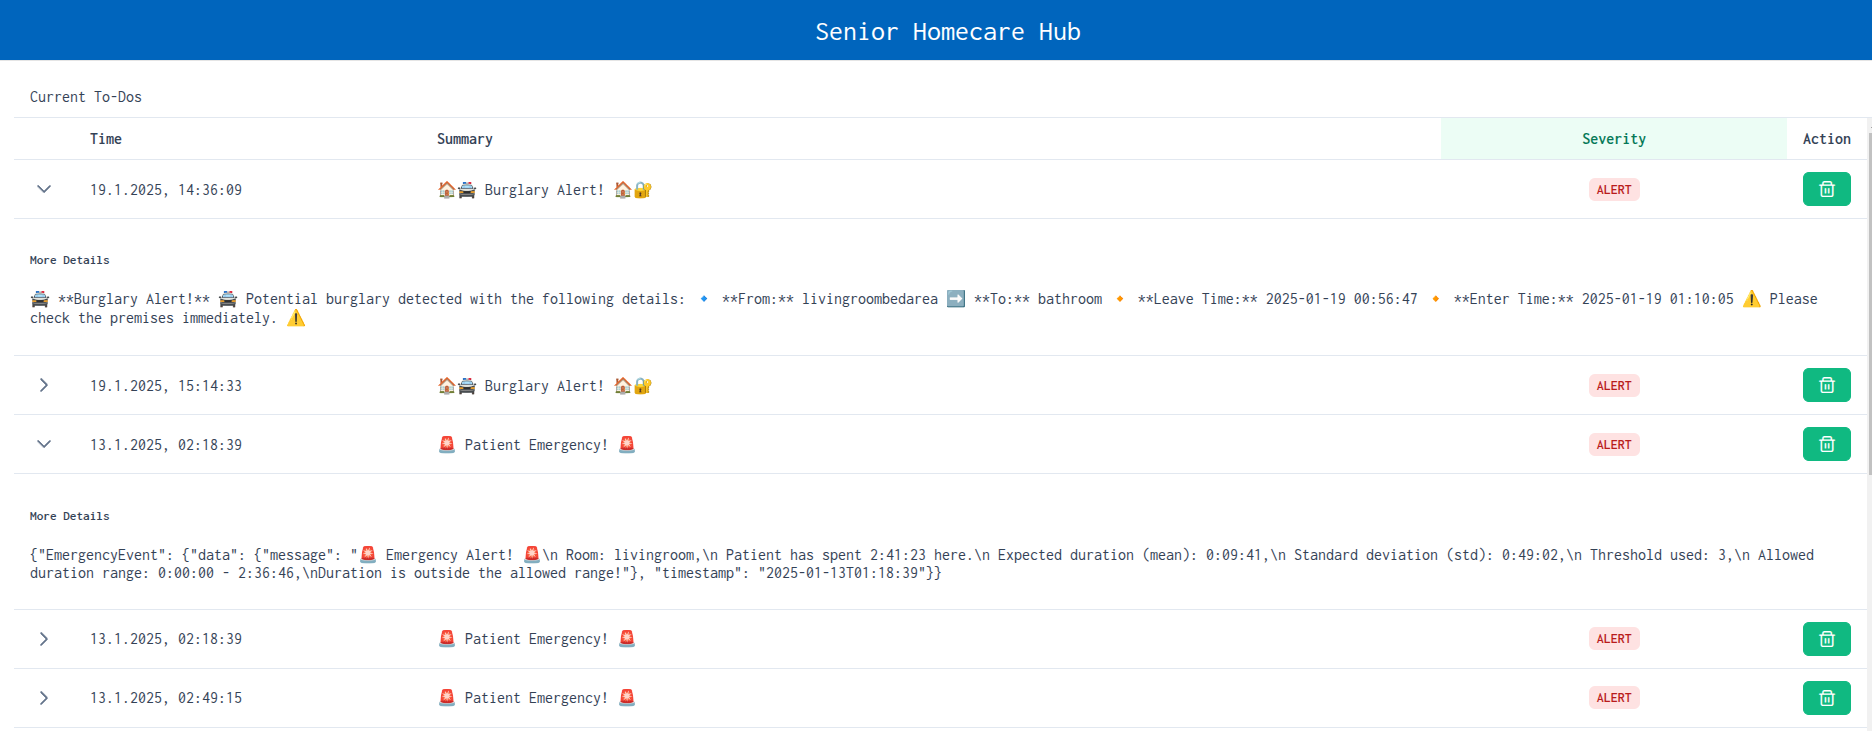
\includegraphics[width=1.1\textwidth]{homecare-hub02.png}
	\caption{The communication with the homecare-hub. Patient emergiencies and burglaries.}
	\label{fig:hub}
\end{figure}

\subsection{ Performance Analysis (2p)}

\subsubsection{Performance Statistics of Emergency Model}

\begin{table}[H]
\centering
\begin{tabular}{@{}lcccc@{}}
\toprule
\textbf{Operation} & \textbf{Mean (s)} & \textbf{Std Dev (s)} & \textbf{Min (s)} & \textbf{Max (s)} \\
\midrule
Fetch/Preprocess Times   & 0.670 & 0.161 & 0.536 & 1.132 \\
Train Times   & 0.014 & 0.005 & 0.012 & 0.028 \\
Save Model Times    & 0.136 & 0.071 & 0.087 & 0.308 \\
\bottomrule
\end{tabular}
\caption{Summary of Time Statistics for 2000 data points (one week of data)}
\label{tab:performance_stats}
\end{table}

\begin{table}[H]
\centering
\begin{tabular}{@{}lcccc@{}}
\toprule
\textbf{Operation} & \textbf{Mean (s)} & \textbf{Std Dev (s)} & \textbf{Min (s)} & \textbf{Max (s)} \\
\midrule
Fetch/Preprocess Times   & 1.993 & 0.248 & 1.685 & 2.492 \\
Train Times   & 0.013 & 0.001 & 0.012 & 0.015 \\
Save Model Times    & 0.118 & 0.047 & 0.082 & 0.235 \\
\bottomrule
\end{tabular}
\caption{Summary of Time Statistics for 28183 Data Points (Full Dataset)}
\label{tab:performance_stats_28183}
\end{table}

\subsubsection{Performance Statistics of Motion Model}

\begin{table}[H]
\centering
\begin{tabular}{@{}lcccc@{}}
\toprule
\textbf{Operation} & \textbf{Mean (s)} & \textbf{Std Dev (s)} & \textbf{Min (s)} & \textbf{Max (s)} \\
\midrule
Fetch/Preprocess Times   & 0.720 & 0.123 & 0.428 & 1.243 \\
Train Times         & 0.803 & 0.202 & 0.708 & 1.400 \\
Save Model Times    & 0.173 & 0.062 & 0.118 & 0.326 \\
\bottomrule
\end{tabular}
\caption{Summary of Time Statistics for Motion Model (2000 Data Points)}
\label{tab:motion_model_stats_2000}
\end{table}

\begin{table}[H]
\centering
\begin{tabular}{@{}lcccc@{}}
\toprule
\textbf{Operation} & \textbf{Mean (s)} & \textbf{Std Dev (s)} & \textbf{Min (s)} & \textbf{Max (s)} \\
\midrule
Fetch/Preprocess Times   & 1.825 & 0.327 & 1.421 & 2.727 \\
Train Times         & 2.906 & 0.289 & 2.625 & 3.727 \\
Save Model Times    & 0.527 & 0.075 & 0.390 & 0.635 \\
\bottomrule
\end{tabular}
\caption{Summary of Time Statistics for Motion Model (28183 Data Points)}
\label{tab:motion_model_stats_28183}
\end{table}

\subsubsection*{Performance Statistics of Burglary Model}

\begin{table}[H]
\centering
\begin{tabular}{@{}lcccc@{}}
\toprule
\textbf{Operation} & \textbf{Mean (s)} & \textbf{Std Dev (s)} & \textbf{Min (s)} & \textbf{Max (s)} \\
\midrule
Fetch/Preprocess Times   & 1.990 & 0.244 & 1.682 & 2.489 \\
Train Times   & 0.013 & 0.001 & 0.012 & 0.015 \\
Save Model Times    & 0.118 & 0.046 & 0.082 & 0.235 \\
\bottomrule
\end{tabular}
\caption{Summary of Time Statistics for Burglary Model (2000 Data Points)}
\label{tab:burglary_model_stats_2000}
\end{table}

\begin{table}[H]
\centering
\begin{tabular}{@{}lcccc@{}}
\toprule
\textbf{Operation} & \textbf{Mean (s)} & \textbf{Std Dev (s)} & \textbf{Min (s)} & \textbf{Max (s)} \\
\midrule
Total Times         & 2.926 & 0.141 & 2.745 & 3.222 \\
\bottomrule
\end{tabular}
\caption{Summary of Time Statistics for Burglary Model (28183 Data Points)}
\label{tab:burglary_model_stats_28183}
\end{table}

\subsubsection{Model Sizes}

The table below summarizes the sizes of different models with calculated mean and standard deviation values.

\begin{table}[h!]
\centering
\begin{tabular}{@{}lcccc@{}}
\toprule
\textbf{Model} & \textbf{Size (Mean)} & \textbf{Size (Std Dev)} & \textbf{Size (Min)} & \textbf{Size (Max)} \\
\midrule
Burglary Model      & 2.2 MiB  & 0.0 MiB  & 2.2 MiB  & 2.2 MiB  \\
Motion Model        & 466.7 KiB & 0.0 KiB & 466.7 KiB & 466.7 KiB \\
Occupancy Model     & 193.25 B & 5.14 B & 188.0 B & 199.0 B \\
\midrule
\bottomrule
\end{tabular}
\caption{Summary of Model Sizes}
\label{tab:model_sizes}
\end{table}

\subsubsection{Performance Statistics of Emergency Model}

\begin{itemize}
    \item Measure response times (time from triggering the event fabric until delivering the event to the scheduler or time from calling the event fabric until actuation communicates an emergency) and execution times (time taken from dispatching the invocation until completing the invocation) for each event. Break it down in terms of fetching data from storage and compute times. From the function trigger to the function call, it is 0.001s (which is negligible). The other times are measured above.
\begin{minted}[fontsize=\small]{python}
# Example of logs
2025-01-19T07:26:30.340Z |       INFO   Function create_burglary_model_function called.
2025-01-19T07:26:30.341Z |       INFO   Received data: {'TrainBurglaryModelEvent': {'data': {'message': 
2025-01-19T07:26:30.341Z |              'Retraining the burglary model'}, 'timestamp': 
2025-01-19T07:26:30.341Z |              '2025-01-19T07:26:30'}}
2025-01-19T07:26:31.943Z | Model training completed.
\end{minted}
\end{itemize}


\subsubsection{Performance with Increasing Data}
As data volume increases, performance scales linearly for operations such as fetching/preprocessing and saving models. This is evident from Tables above.

\begin{itemize}
    \item \textbf{Example Correlation:}
    \begin{itemize}
        \item Preprocessing time for 2000 data points: ~0.670s (mean).
        \item Preprocessing time for 28183 data points: ~1.993s (mean), scaling directly with data size.
    \end{itemize}
\end{itemize}

\subsubsection{Preprocessing vs. Training Ratio}
The ratio of preprocessing time to training time highlights the dominant cost in overall execution:

\begin{itemize}
    \item \textbf{Emergency Model:}
    \begin{itemize}
        \item Preprocessing to Training Ratio (2000 points): \( \frac{0.670}{0.014} \approx 47.86 \)
        \item Preprocessing to Training Ratio (28183 points): \( \frac{1.993}{0.013} \approx 153.31 \)
    \end{itemize}
    \item \textbf{Motion Model:}
    \begin{itemize}
        \item Preprocessing to Training Ratio (2000 points): \( \frac{1.990}{0.803} \approx 2.48 \)
        \item Preprocessing to Training Ratio (28183 points): \( \frac{1.993}{2.906} \approx 0.69 \)
    \end{itemize}
\end{itemize}

\subsection{Limitations (1p)}

The current system has several limitations:
\begin{itemize}
    \item The behavioral models assume only one person, which isn't ideal for multiple occupants. It needs consistent network connectivity, and offline periods can cause data delays or loss.
    \item The burglary detection might give false alarms due to normal activities like having guests.
    \item The current solution also lacks the path analyses and the burglary detection model is trained on transation data, not paths. Thee visualisation in homecare hub is not ideal and could be improved.
    \item The occupancy model could be further devided into separated times during the day.
\end{itemize}
\subsection{Code Structure (2p)}
\label{sec:code_structure}

This project---named \textit{Digital Twin App}---is split into separate folders for each major component: 
\texttt{actuation}, \texttt{modeling},\texttt{monitoring}, \texttt{viz-component} and \texttt{homecare-hub}. Each folder contains a \texttt{main.py} file
that implements logic specific to that component.
A common \texttt{base/} folder (copied into each component) provides shared utilities 
such as event classes, triggers, and helper functions to interact with databases, object storage, 
and the HomeCare Hub utils to send the info and todo messages.

For additional information also refer to the README.md file in the code repository. (There is one common file and then also separate README.md files in each component folder.)

\begin{itemize}
  \item \textbf{Individual Folders per Component}
  \begin{itemize}
    \item \texttt{actuation/}
      \begin{itemize}
        \item \texttt{main.py}: Defines and deploys \texttt{create\_emergency\_notification\_function}
          and \texttt{create\_burglary\_notification\_function}, each responsible for generating 
          notifications (e.g., via \texttt{send\_todo}) when emergencies or burglaries are detected.
        \item \texttt{Dockerfile}: Builds and containers this microservice.
      \end{itemize}

    \item \texttt{modeling/}
      \begin{itemize}
        \item \texttt{main.py}: Exposes endpoints for training the Occupancy, Motion, 
          and Burglary ML models. Internally uses local modules like \texttt{occupancy\_model.py},
          \texttt{motion\_model.py}, and \texttt{burglary\_model.py}.
        \item \texttt{occupancy\_model.py}: Responsible for preparing and training the occupancy model, 
          computing room-stay durations, etc.
        \item \texttt{motion\_model.py}: Contains logic for analyzing transitions and motion events. 
        \item \texttt{burglary\_model.py}: Implements an Isolation Forest-based burglary-detection model.
      \end{itemize}

    \item \texttt{monitoring/}
      \begin{itemize}
        \item \texttt{main.py}: Registers asynchronous functions for checking emergencies 
          (\texttt{check\_emergency\_detection\_function}), burglary events 
          (\texttt{check\_burglary\_detection\_function}), and general motion analysis 
          (\texttt{motion\_analysis\_function}). Also configures periodic triggers for each event 
          based on intervals specified in \texttt{config.py}.
        \item \texttt{config.py}: Defines environment variables and intervals 
          (e.g., \texttt{TRAIN\_OCCUPANCY\_MODEL\_INTERVAL = "168h"}, 
          \texttt{CHECK\_EMERGENCY\_INTERVAL = "30m"}). These parameters are adjustable 
          to match user needs.
      \end{itemize}
  \end{itemize}

  \item \textbf{Common \texttt{base/} Folder}
  \begin{itemize}
    \item \texttt{gateway.py}: Offers the \texttt{LocalGateway} class, enabling the components to define 
      endpoints in a consistent manner.
    \item \texttt{event.py}: Contains all event classes (e.g., \texttt{TrainOccupancyModelEvent}, 
      \texttt{CheckEmergencyEvent}, \texttt{BurglaryEvent}), used for the event-driven architecture.
    \item \texttt{trigger.py}: Implements \texttt{PeriodicTrigger} and \texttt{OneShotTrigger} for scheduling 
      or one-time event invocation.
    \item \texttt{homecare\_hub\_utils.py}: Provides communication methods like \texttt{send\_info} 
      (for general notifications) and \texttt{send\_todo} (for alerts needing user action).
    \item \texttt{influx\_utils.py}: Defines \texttt{fetch\_all\_sensor\_data} and other functions to 
      query InfluxDB for sensor, battery, or aggregated data.
    \item \texttt{minio\_utils.py}: Manages saving/loading DataFrames (model results, stats) to/from MinIO object storage.
  \end{itemize}
\end{itemize}

\paragraph{Challenges and Organization Choices.}
Initially, I had some confusion on how to structure the code for different services (e.g.\ 
\texttt{actuation} vs.\ \texttt{monitoring}). I also had to learn how to keep track of
common logic in the \texttt{base/} folder so I would not duplicate code in each microservice. 

I found Docker and Kubernetes orchestration somewhat complex at first, but following 
the microservices approach allowed me to build and deploy each component independently. 
This structure made debugging easier: if something failed in \texttt{monitoring}, it rarely 
affected \texttt{actuation} or \texttt{modeling} directly. Additionally, relying on 
\texttt{docker-compose} or \texttt{k8s/} manifests simplified local testing.

\section{Declaration of data usage}

Specify, whether you allow us to keep your data for tests with our own implementation. We make sure, that the data cannot be tracked down to your name. 

\subsection{Data Donation Agreement}
Under this agreement, you understand that we, the Chair CAPS, can use (read, modify, delete) any sensor data generated during the WiSe2024 in future research and educational activities or produce derivative works. Given the current structure of the stored data in the procured Raspberry Pi, we ensure the data cannot reveal any personal information of the donor as it refers to a generic user: \texttt{iot-user}, while the fields contain generic names and values.
\bigskip
\\
\\

\noindent\rule{5cm}{0.4pt} \hfill \noindent\rule{5cm}{0.4pt}\\
MTK, Signature \hfill Date, Place

\pagebreak

% Put citations from bibtex into References section which were not
% explicity cited.
\nocite{robotron,
stonx,vice,650sim,herculessim,zib,4004,thermal1,thermal2,rojas}


\bibliographystyle{plain}
% Literature sources are to be found in seminarpaper.bib
\bibliography{iot_report}
\end{document}
